\documentclass[utf8, diplomski, english, numeric]{fer}
\usepackage{booktabs}
\usepackage{caption}
\usepackage{subcaption}
\usepackage{graphicx}
\usepackage{grffile}
\usepackage{listings}
\usepackage[table,xcdraw]{xcolor}
\usepackage{multirow}
\usepackage{dirtree}
\usepackage{float}
\usepackage[hidelinks]{hyperref}
\usepackage[utf8]{inputenc}
\usepackage[english]{babel}
\usepackage[fixlanguage]{babelbib}
\usepackage[outputdir=build]{minted}
\usepackage{todonotes}
\usepackage[title]{appendix}

\lstset{
basicstyle=\small\ttfamily,
columns=flexible,
breaklines=true
}

\newcommand{\todoi}[1]{\todo[inline]{#1}}

\newcommand{\code}[1]{\texttt{#1}}

\def\changemargin#1#2{\list{}{\rightmargin#2\leftmargin#1}\item[]}
\let\endchangemargin=\endlist 

\begin{document}

\thesisnumber{1981}

\title{Software and Hardware Architecture for Redundant Embedded Systems}

\author{Dino Šarić}

\maketitle

\izvornik
%\includepdf[pages={1-}]{izvornik.pdf}

\zahvala{Thanks to my parents for supporting me financially and giving me an opportunity of studying away from home. Thanks to my aunt Dijana and my friends for supporting me emotionally. 

Thanks to my mentor izv. prof. dr. sc. Hrvoje Džapo and his assistant Ivan Pavić mag. ing. for a friendly, fast and diligent approach during the studies and the writing of the thesis. Thanks to all the helpful current and former students from the college forums. Finally, thanks to the YouTubers that made understanding the college curriculum much easier.} % Gramarly OK

\tableofcontents
\listoffigures
\listoftables

\chapter*{Introduction} 

In a world with increasing number of electronic systems in hazardous environment, the correct operation of active systems is ever more important for ensuring less catastrophes. In year 2000, Air France Concorde flight crashed soon after its take-of killing 113 people, in 2005 Texas City refinery exploded killing 15 people and injuring 180. Similar disasters to these were the motivation for the  creation of functional safety principles. 
\begin{figure}[H]
    \centering
    \begin{minipage}{.5\textwidth}
          \centering
          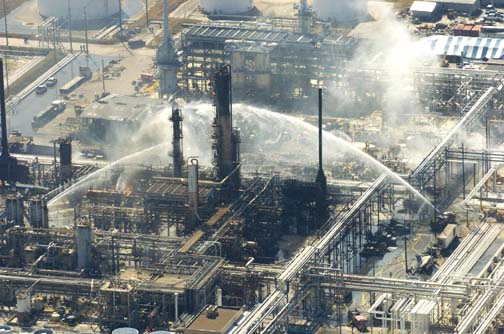
\includegraphics[width=.7\linewidth]{images/texas_refinery.jpg}
          \captionof{figure}{Texas refinery disaster}
          \label{fig:texas_refinery}
    \end{minipage}%
    \begin{minipage}{.5\textwidth}
          \centering
          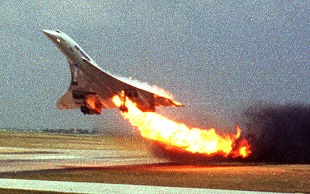
\includegraphics[width=.74\linewidth]{images/concorde_disaster.jpg}
          \captionof{figure}{ Air France Concorde disaster}
          \label{fig:concorde_disaster}
    \end{minipage}
\end{figure}

Functional safety is the part of the overall safety that depends on a system or equipment operating correctly in response to its inputs.\cite{func_safety_brief} In other words, the goal of functional safety is ensuring even when the system fails its response is predictable and safe. Today, the concept of functional safety is part of everyday life and applies to every industry one can think of. For example, functional safety ensures that airbags in a car instantly deploy during impact to protect the passengers. Another good example is an automated flight control system in the airplanes. Autopilot controls pitch and roll of the aircraft changing the heading and altitude, all of which is developed with respect to functional safety parameters, activating alarms and other measures when they are breached.\cite{func_safety_brief}

Motivation of this paper is exploring how are principles of functional safety applied to the engineering projects. Investigate how and why redundancy is implemented in hardware and software. As a part of that, redundant microcontrollers are explored and compared to non-redundant counterparts. Additionally, functional safety additions to FreeRTOS operating system are implemented. Modifications add task replication and a option to measure execution time of tasks. Finally, secure bootloader is added, bootloader has a command shell interface and has option of updating the current application.

The thesis is organized in the following way:

\begin{itemize}

    \item \autoref{functional_safety} gives brief introduction of functional safety process. Moreover, chapter gives a overview of how is hardware of embedded systems designed to support redundancy,
    \item \autoref{cortex_r_additions} investigates ARM Cortex R microcontroller's inner workings and what do they add over Cortex M,
    \item \autoref{freertos_kernel} gives overview of of FreeRTOS and inner workings of tasks, scheduler and timers,
    \item \autoref{freertos_modification} gives overview of added safety functions to the FreeRTOS kernel,
    \item \autoref{custom_bootloader} explains how the developed secure bootloader functions and its features and
    \item \autoref{demonstration} demonstrates the functionality of the developed software.
    
\end{itemize}
   
\chapter{Functional safety in embedded systems}
\label{functional_safety}

\section{IEC standards}

A variety of standards exist for specific or general markets, to facilitate the compliance of the systems to the functional safety principles. The standard IEC 61508 gives methods on how to apply, design, deploy and maintain automatic protection systems called safety-related systems.
Along with the more general standard, industry specific standards exist:
\begin{itemize}

    \item ISO 26262 for automotive passenger vehicles,
    \item IEC 61511 for the process industry and associated instrumentation,
    \item EN 50128 for software development of railway applications,
    \item IEC 61513 for nuclear power plants,
    \item IEC 62061 and ISO 13849 for machinery electrical control systems,
    \item IEC 62304 for medical systems and
    \item IEC 60730 for white goods.

\end{itemize}

Mentioned standards provide guidelines to assess rick and assign safety goals for safety-related systems of various industries. They provide frameworks for quantitative analysis of random failure rates and effectiveness of diagnostics to detect them. They also provide guidelines for maintenance of the safety-related systems after the deployment.

IEC 61508 is a basic functional safety standard applicable to all kinds of industry. It defines functional safety as: “part of the overall safety relating to the EUC (Equipment Under Control) and the EUC control system which depends on the correct functioning of the Electrical/Electronic/Programmable Electronic Safety-related Systems (E/E/PE) safety-related systems, other technology safety-related systems and external risk reduction facilities.” The fundamental concept is that any safety-related system must work correctly or fail in a predictable (safe) way. Functional safety relies only on active systems, and safety measures that rely on passive systems are not functional safety. \citep{func_safety_explained}

\section{Terminology}


\todoi{Functional safety terminology, SIL, SIF, SIS...}

\section{Certification process}

\todoi{Procjena etc.}

\section{Embedded processors redundancy - lockstep}

Consider a system with one processing unit. Such system is obviously non-redundant from the
aspect of instruction execution. Lockstep is redundancy mechanism for increasing the system reliability
by introducing at least one redundant processing unit. Redundant processing unit replicates the behavior of
the original processing unit. Depending on number of processing units lockstep can provide fault-detection, if there are less than three processing units in a system, or both fault-detection and
fault-tolerance with more than two processing units in a system. \citep{ipavic_lockstep}

Locksteped processors can get upto SIL3, but not SIL4 as a use of on-chip redundancy is limited by IEC 61508 standard to SIL3. Therefore, although it may seem, lockstep is certainly not panacea in all safety systems and certain amount of work is needed to justify its usage. Nevertheless, for all safety integrity levels, but SIL4 lockstep is often used extensively (e.g. automotive applications). \citep{ipavic_lockstep}
\chapter{ARM Cortex-R functional safety additions over ARM Cortex-M}
\label{cortex_r_additions}

\section{ARM Cortex-R introduction}

The ARM Cortex-R is a family of 32-bit RISC processors. The cores are optimized for hard real-time and safety-critical applications. Cortex-R family consists of ARM Cortex-R4(F), ARM Cortex-R5(F), ARM Cortex-R7(F), ARM Cortex-R8(F and ARM Cortex-R52(F).

The Cortex-R is suitable for use in computer-controlled systems where very low latency and/or a high level of safety is required. An example of a hard real-time, safety-critical application would be a modern electronic braking system in an automobile. The system not only needs to be fast and responsive to a plethora of sensor data input but is also responsible for human safety. A failure of such a system could lead to severe injury or loss of life. Other examples of hard real-time and safety-critical applications include medical devices, electronic control units (ECU), robotics, etc.

\section{ARM Cortex-M introduction}

The ARM Cortex-M is also a family of 32-bit RISC processors. The cores are optimized for low-cost and energy-efficient microcontrollers. These cores are being used in tens of billions of consumer devices. The processors are intended for deeply embedded applications that require fast interrupt response features \citep{cortex_m4_reference}. The family consists of Cortex-M0, Cortex-M0+, Cortex-M1, Cortex-M3, Cortex-M4, Cortex-M7, Cortex-M23, Cortex-M33, Cortex-M35P and Cortex-M55.


\section{ARM Cortex-R processor lockstep}

\subsection{Dual core lockstep}

A Cortex-R5 processor group has four configurations, as described in \citep{cortex_r5_reference_manual}:
\begin{itemize}

    \item single CPU,
    \item twin CPU,
    \item redundant CPU and
    \item split/lock configuration.
    
\end{itemize}

Twin CPU configuration includes two individual and decoupled CPUs. Each CPU has its own
cache RAMs, debug logic and bus interfaces to the rest of the SoC. It
offers higher performance than a standard single CPU configuration. 

In redundant CPU configuration (lockstep), there is a functional CPU and a second redundant copy of the majority of the CPU logic. The redundant logic is driven by the same inputs as the functional logic.  In particular, the redundant CPU logic shares the same cache RAMs as the functional CPU. Therefore only one set of cache RAMs is required. The redundant logic
operates in lock-step with the CPU but does not directly affect the processor behavior in any way \citep{cortex_r5_reference_manual}. The CPU outputs to the cache RAMs are driven \textbf{exclusively} by the functional CPU. The comparison logic for comparing the outputs of the redundant logic and the functional logic can detect a single fault that occurs in either set of logic. ARM provides example comparison logic, but the developer can change it during the implementation. 

Split/lock configuration is a combination of two previously mentioned configurations. This mode includes two processors. If a processor is in split mode the CPUs work in twin CPU configuration, and if the processor is in lock mode it is in a redundant configuration.

\begin{figure}[H]

      \centering
      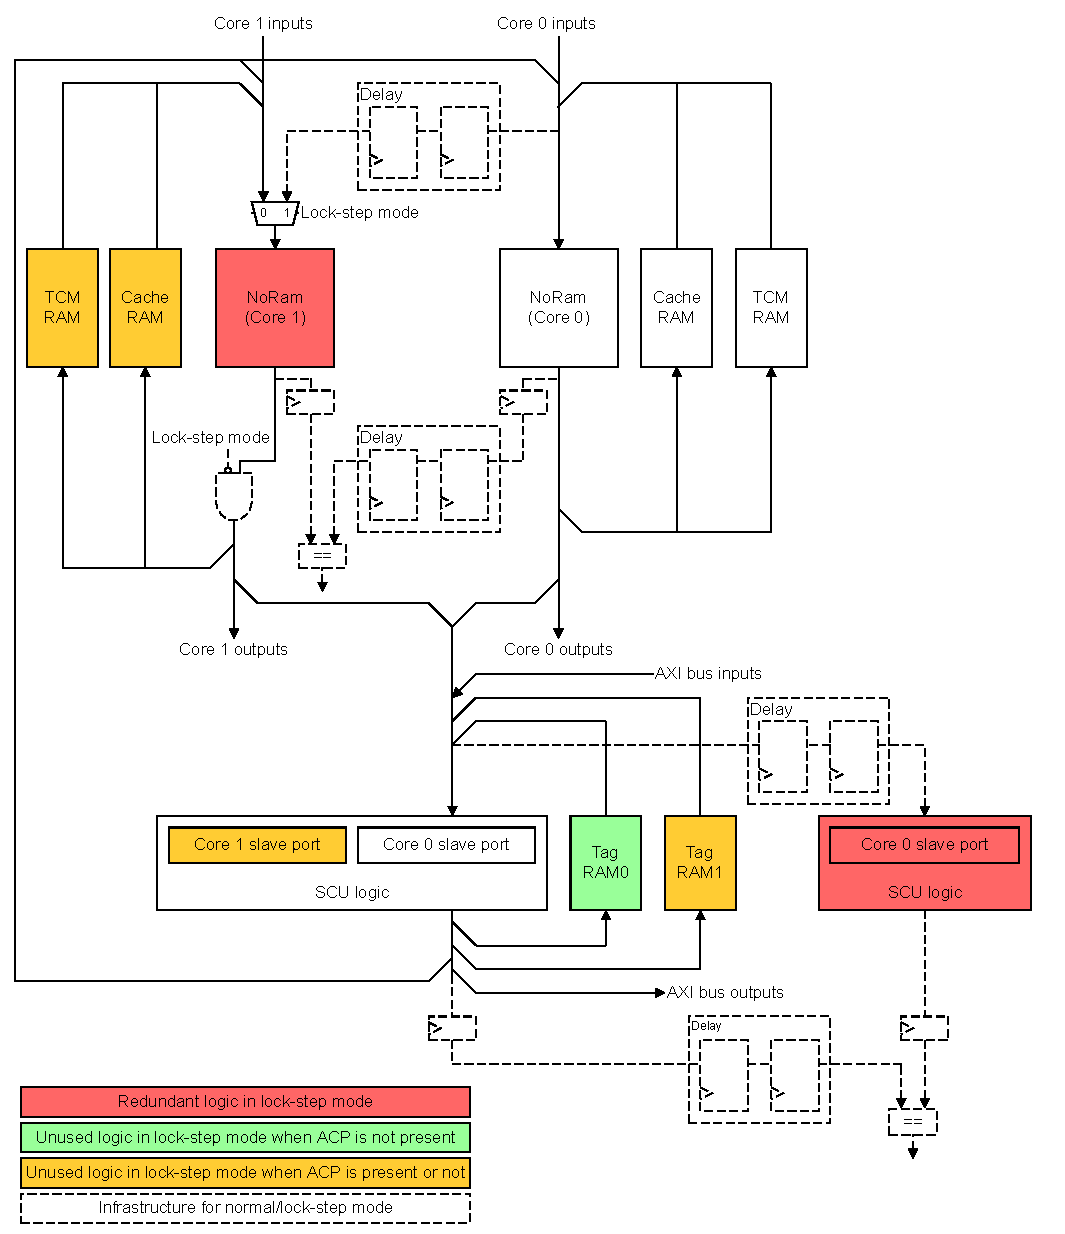
\includegraphics[width=1\linewidth]{images/split_lock_configuration.png}
      \caption{Split/lock configuration \citep{cortex_r8_reference_manual}}
      \label{fig:split_lock_configuration}
    
\end{figure}

\subsection{Triple core lockstep}

ARM triple-core lockstep architecture (TCLS) builds upon the industry success of the ARM Cortex-R5 dual-core lock-step (DCLS). The TCLS architecture adds a third redundant CPU unit to the DCLS Cortex-R5 system to achieve fail functional capabilities and hence increase the availability of the system \citep{TCLS_cortex_r}.

Cores in triple lockstep have shared data and instruction cache, but each Cortex-R5 has its own clock tree. \autoref{fig:tcls_architecture} shows the system level solution to mitigate soft errors occurring in the redundant CPUs. On the right side of the figure, the TCLS assist unit is visualized. TCLS assist unit supports the lockstep functioning of the CPUs and handles the error recovery process. The unit consists of a majority voter, error detection logic and synchronization logic.


\begin{figure}[H]

      \centering
      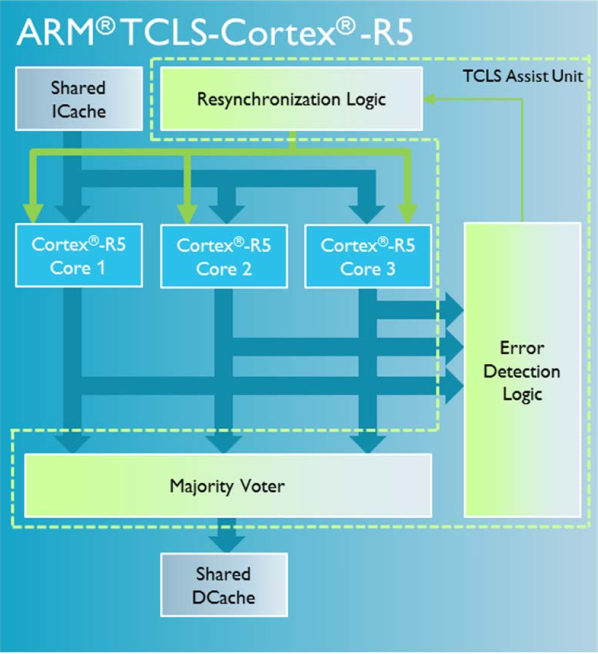
\includegraphics[width=0.7\linewidth]{images/tcls_architecture.png}
      \caption{ARM triple core lockstep of Cortex-R5 \citep{TCLS_cortex_r}}
      \label{fig:tcls_architecture}
    
\end{figure}

At every clock cycle, the instructions to execute are read
from the shared instruction cache or TCM (tightly coupled memory) and distributed to
the triplicated CPUs. The outputs from the CPUs are majority voted and
forwarded to the shared data cache, TCM, and I/O ports.
Simultaneously, the Error Detection logic checks if there is any
mismatch in the outputs delivered by the three CPUs. If there is
a mismatch, all CPUs are interrupted and the Error Detection
logic identifies whether it is a correctable error (i.e., only one
of the CPUs delivers a different set of outputs) or an
uncorrectable one (i.e., all CPUs deliver different outputs). If
the error is correctable, the TCLS passes the control to the
resynchronization logic to correct the architectural state of the
erroneous CPU, that is, to resynchronize all the CPUs. Note
here that the Majority Voter acts as an error propagation
boundary, preventing correctable errors from propagating to
memories and I/O ports. In the highly unlikely case that the
error is uncorrectable, the TCLS transitions to a fail-safe
operation state \citep{TCLS_cortex_r}.

As mentioned in the last paragraph, the majority voter is in the critical path of the system, but the error detection logic is out of the critical path and is pipelined to increase performance.

\autoref{fig:tcls_resynchronization} show the flow diagram of the resynchronization logic. Upon a correctable error is detected, the resynchronization logic can immediately trigger the CPU resynchronization process. This action prevents the interruption of critical real-time tasks. It should be noted that the system can continue working on two remaining CPUs, which are in a functionally correct state. The third CPU is recovered from the two functioning CPUs. Unlike the dual-core lockstep, the recovery of the triple-core lockstep is automatic and transparent to the software \citep{TCLS_cortex_r}.

\begin{figure}[H]

      \centering
      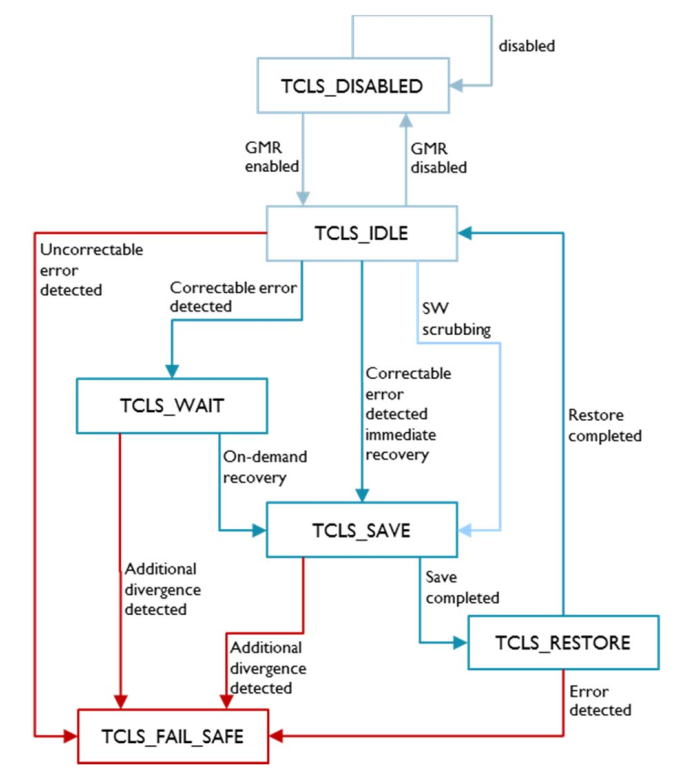
\includegraphics[width=0.9\linewidth]{images/tcls_resynchronization.png}
      \caption{TCLS resynchronization finite state machine \citep{TCLS_cortex_r}}
      \label{fig:tcls_resynchronization}
    
\end{figure}

\section{RAM error correction}

In microcontrollers, stray radiation and other effects can cause the data stored in RAM (random access memory) to be corrupted (bit flip).  The tightly coupled memories (TCMs) and caches on a Cortex-R processor can be configured to detect and correct errors that can occur in the RAMs. Extra, redundant data (checksum) is computed by the processor and stored in RAMs alongside the real data. When the processor reads the data from the RAM, it checks the redundant data matches the real data and can either signal an error, or attempt to correct the data.

Cortex-R5 allows the usage of:
\begin{itemize}

    \item parity,
    \item 64-bit ECC or
    \item 32-bit ECC \citep{cortex_r5_reference_manual}.
\end{itemize}

With parity, an error can be detected, but it can't be corrected. Using either 64-bit or 32-bit ECC (error checking and correction) detects up to two errors in a data chunk (either 64-bit or 32-bit) and correct any single error in the data chunk. Parity adds one redundant bit for every byte. 64-bit ECC adds one byte per 8-byte data chunk. 32-bit ECC adds seven bits per 4 bytes of the data chunk. 

Cortex-R8 uses 32-bit, 34-bit or 64-bit ECC of variable data chunks to protect its RAMs \citep{cortex_r8_reference_manual}.

\section{Interrupt handling}

According to \citep{cortex_r5_reference_manual}, Interrupt handling in the processor is compatible with previous ARM architectures, but has
several additional features to improve interrupt performance for real-time applications.

ARM Cortex-R5 connects the vectored interrupt controller (VIC) over a port, unlike ARM Cortex-M series microcontrollers that only have VIC close to the core. Having a VIC over the port provides faster interrupt entry, but one can disable it for compatibility with earlier interrupt controllers \citep{cortex_r5_reference_manual}. ARM Cortex-R5 doesn't allow tail chaining of the interrupts, nor the handling of late-arriving interrupts, unlike ARM Cortex-M series. 

Both ARM Cortex-R and Cortex-M series microcontrollers can abandon assembler instructions LDM and STM to lower the interrupt's latency. While Cortex-R microcontrollers will rerun the whole command upon the return from the interrupt, the ARM Cortex-M microcontrollers will just continue where they left of.

 

\section{CPU Compare Module for Cortex-R5F by Texas Instruments}

CPU compare module (CCM) detects run-time faults in devices like the CPU and VIM (vectored interrupt controller module) and forwards them to the next step in the error handling of the microcontroller i.e. to ESM (error signaling module). Alongside the run-time fault testing, CCM incorporates a self-test capability to allow for boot time checking of hardware faults within the CCM itself \citep{TMS570LS31x21x_manual}.

The main features of the CCM are:
\begin{itemize}

    \item{run-time detection of faults,}
    \item{self-test capability and}
    \item{error forcing capability.}

\end{itemize}

There are four modes of diagnostics for CPU/VIM output compare.
\begin{itemize}

    \item active compare lockstep,
    \item self-test,
    \item error forcing and
    \item self-test error forcing mode.

\end{itemize}

Active compare lockstep mode is defaulted to on start-up. The bus output signals of both CPU and VIMs are compared. List of all compared output signals is available in \citep[p. 500]{TMS570LS31x21x_manual}.

In self-test mode, test patterns are automatically generated by the CCM-R4F to
determine its correct functionality. In case of error detection that indicates a
hardware fault on the module itself, a “CCM-R4F - self-test” flag will be raised to
the ESM. After the completion or termination of the self-test, if no error occurred,
the self-test complete flag is set to notify the system to proceed appropriately. The compare match test and compare mismatch test are generated to ensure proper functioning. In compare match test an identical vector is applied to both input ports at the same time expecting a compare match. The compare mismatch test is similar to the compare match test, but one of the input vectors has one bit flipped. On the output, compare mismatch is expected.

Error forcing mode ensures that an error on the CCM's input is detected. In the case when the error from error forcing mode is not detected there is a hardware failure present. The difference between the compare mismatch test and error forcing mode is that error forcing mode ensures that compare error output signal asserts. This mode lasts for one CPU cycle.

\chapter{FreeRTOS kernel}
\label{freertos_kernel}

\section{Introduction}

FreeRTOS is a real-time operating system kernel (RTOS) for embedded devices. It has been ported to 35 microcontroller pletforms and has MIT open source licence hence the free in the name. \citep{freertos_licence}

Operating system (OS) is designed to be small and simple. The kernel itself has only three C files. It is written mostly in C with some assembly code included for the scheduler routines.

FreeRTOS is ideally suited for deeply embedded real-time applications that use
microcontrollers or small microprocessors. This type of application normally includes a mix of
both hard and soft real-time requirements. \citep{freertos_mastering}

Soft real-time requirements are those that state a time deadline—but breaching the deadline
would not render the system useless. For example, responding to keystrokes too slowly might
make a system seem annoyingly unresponsive without actually making it unusable. \citep{freertos_mastering}

Hard real-time requirements are those that state a time deadline—and breaching the deadline
would result in absolute failure of the system. For example, a driver’s airbag has the potential
to do more harm than good if it responded to crash sensor inputs too slowly. \citep{freertos_mastering}

\noindent FreeRTOS features:

\begin{itemize}
    
    \item Pre-emptive or co-operative operation
    \item Very flexible task priority assignment
    \item Flexible, fast and light weight task notification mechanism
    \item Queues
    \item Binary and counting semaphores
    \item Mutexes
    \item Recursive mutexes
    \item Software timers
    \item Event groups
    \item Tick hook functions
    \item Idle hook functions
    \item Stack overflow checking
    \item Trace recording
    \item Task run-time statistics gathering
    \item Optional comemercial licensing and support
    \item Full interrupt nesting model (on some architectures)
    \item Tick-less capability for extreme low power applications
    \item Software manages interrrupt stack when appropriate (could save RAM space)
    
\end{itemize}

\noindent FreeRTOS file structure is shown in \autoref{fig:freertos_structure}.

\begin{figure}[H]
\dirtree{%
.1 Source.
.2 include.
.3 FreeRTOS.h.
.3 list.h - Primary structure used inside the kernel.
.3 message\textunderscore buffer.h.
.3 portable.h.
.3 projdefs.h.
.3 queue.h.
.3 semphr.h - Semaphores.
.3 stream\textunderscore buffer.h.
.3 task.h.
.3 timers.h - Software timers. 
.2 portable.
.3 [compiler] e.g{. GCC}.
.4 [architecture] e.g{. ARM\textunderscore CM4F}.
.5 port.c - Architecture and compiler specific.
.5 portmacro.c.
.3 MemMang.
.4 heap\textunderscore X.c - X is a heap number used.
.2 croutine.c.
.2 event\textunderscore groups.c.
.2 list.c.
.2 queue.c.
.2 stream\textunderscore buffer.c.
.2 tasks.c - Tasks and scheduler implementation.
.2 timers.c.
}
\caption{FreeRTOS file structure}
\label{fig:freertos_structure}
\end{figure}

\section{Inner workings of the tasks}
 

Every FreeRTOS task has a stack and a task control block, or short TCB. Kernel uses the TCB to manage tasks. A TCB contains all information necessary to completely describe the state of a task. \citep{freertos_inner_workings} A FreeRTOS task can exist in five states: running, blocked, ready, suspended and deleted. A state diagram is shown in \autoref{fig:freertos_task_states}.

\begin{figure}[H]

      \centering
      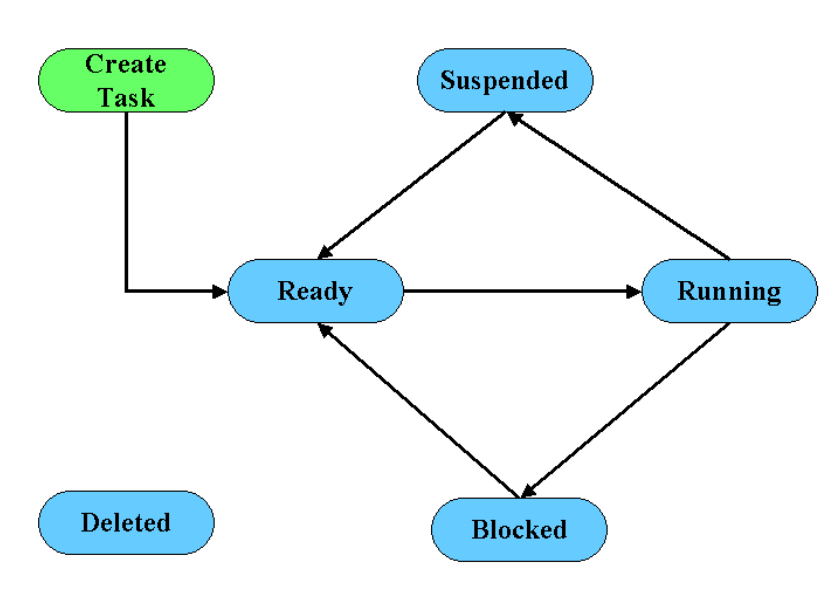
\includegraphics[width=0.7\linewidth]{images/freertos_task_states.png}
      \caption{FreeRTOS task states\citep[p~10]{freertos_inner_workings}}
      \label{fig:freertos_task_states}
    
\end{figure}

When a new task is created its TCB is populated. New tasks are immediately placed in a ready list. Whole scheduling is comprised of a lot of lists.

Ready list is arranged in order of priority with tasks of equal priority being serviced round robin. Ready list is not actually  a single list, rather a configMAX\textunderscore PRIORITIES number of lists. Each priority level has a list for it. When scheduler looks for the next task it walks from the tasks with highest priority to the one with the lowest. Variable pxCurrentTCB points to a process in the ready list that is currently running.

The tasks in FreeRTOS can be blocked when accessing a resource that is not currently available. The scheduler blocks the tasks when they attempt to read from an empty container or write into a full one. This is also true for the semaphores, as they are a queue of size one in the background.

As indicated earlier, access attempts against queues can be blocking or non-blocking.
The distinction is made via the xTicksToWait variable which is passed into the queue
access request as an argument. If xTicksToWait is 0, and the queue is empty/full, the
task does not block. Otherwise, the task will block for a period of xTicksToWait
scheduler ticks or until an event on the queue frees up the resource.

Tasks can also be blocked without a use of containers. FreeRTOS provied vTaskDelay and vTaskDelayUntil functions for this purpose. When a task is delayed it is put onto a delay list. On every tick, scheduler checks if one of the tasks from the delay lists are unblocked. If they are, they are moved to the ready list.

Any task or, in fact, all tasks except the one currently running (and those servicing ISRs)
can be placed in the Suspended state indefinitely. Tasks that are placed in this state are
not waiting on events and do not consume any resource or kernel attention until they are
moved out of the Suspended state. When unsuspended, they are returned to the Ready state.

Finally, tasks can also be deleted. When delete is requested task is put in a deleted state. Deleted state is required because tasks are not deleted immediately after the call. Rather tasks are deleted, and its resources released, from the IDLE task. IDLE task has the lowest possible priority so this job may take some time.

\section{Inner workings of the scheduler}

This section gives a brief overview of a FreeRTOS scheduler.

\autoref{fig:freertos_scheduler_overview} shows an overview of the scheduler algorithm. The scheduler operates as a timer interrupt service routine that is called once every tick. Tick period is defined by configTICK\textunderscore RATE\textunderscore HZ. 

\begin{figure}[H]

      \centering
      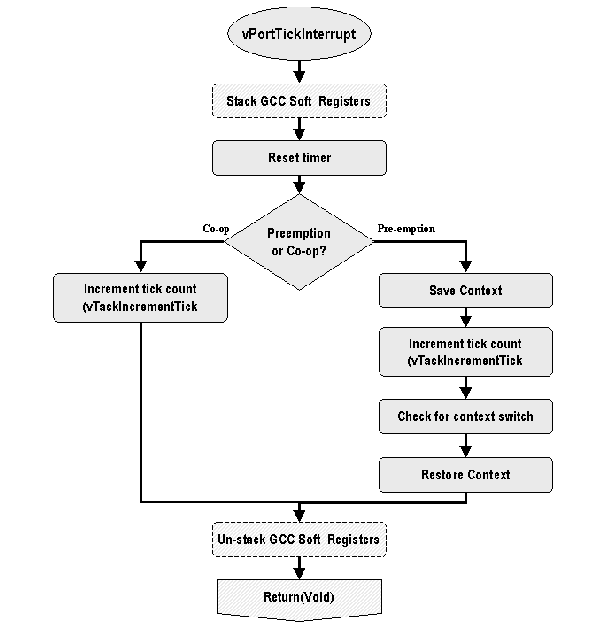
\includegraphics[width=0.8\linewidth]{images/freertos_scheduler_overview.png}
      \caption{Scheduler algorithm\citep[p~20]{freertos_inner_workings}}
      \label{fig:freertos_scheduler_overview}
    
\end{figure}

Context saving is done for the current task. Needed registers are saved on top of the task's stack. It is worth noting, when a task is first created its task is artificially filled. After saving the context scheduler increments the tick and checks if any other task with higher priority has been unblocked, or there is a task with same priority ready. Finally, context is restored and scheduler returns from the interrupt.  

\autoref{fig:freertos_scheduler_increment} shows the algorithm for vTaskIncrementTisk. vTaskIncrementTick is called once each clock tick by the HAL (whenever the timer ISR occurs). The right hand
branch of the algorithm deals with normal scheduler operation while the left hand branch
executes when the scheduler is suspended. As discussed earlier, the right hand branch
simply increments the tick count and then checks to see if the clock has overflowed. If
that’s the case, then the DelayedTask and OverflowDelayedTask list pointers are
swapped and a global counter tracking the number of overflows is incremented. An
increase in the tick count may have caused a delayed task to wake so check is performed.

\begin{figure}[H]

      \centering
      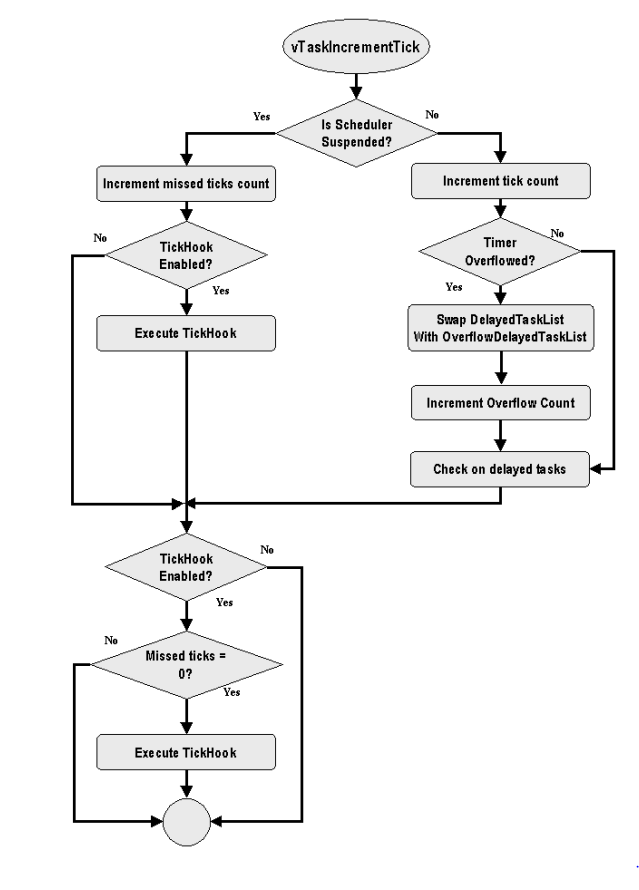
\includegraphics[width=0.8\linewidth]{images/freertos_scheduler_increment.png}
      \caption{vTaskIncrementTick algorithm\citep[p~31]{freertos_inner_workings}}
      \label{fig:freertos_scheduler_increment}
    
\end{figure}

More about the scheduler can be found in \citep{freertos_inner_workings}.

\section{Inner workings of the timers}

Similarly to tasks, FreeRTOS timers have a control block. Timer's control block contains timers period, name, does it auto reload and list item. Active timers are stored in current timer list in order of expiry time, first element is the one that will expire first.

When timers are included from the configuration, scheduler on start up  creates the timer daemon service (its priority is modifiable with configTIMER\textunderscore TASK\textunderscore PRIORITY). Timer daemon has a job of processing the expired timers and receiving the commands. All commands controlling the timers the commands are not sent directly to the requested timer, rather all commands are sent to the queue to be later processed by the timer's daemon.

Timer daemon normally just waits for unblocking of the next timer or a new commands from the queue. When a timer expires daemon is woken up, it processes the timer, checks again for received commands and goes back to waiting. If a new commands has arrived the same is expected, first the commands is processed than the task goes back to waiting.

\chapter{FreeRTOS functional safety additions}
\label{freertos_modification}

\section{Timed tasks addition}

\subsection{Introduction}

Atop of all FreeRTOS functionality ability of measuring task's run time and its total time (running + other states) is not provided. Such feature is extremely useful for hard real-time embedded systems. In such systems breaching the deadline means failure of the system.

Adding the aforementioned timers to the tasks means ability to detect if the task ran for too long or it didn't get enough processor time. When such event has occurred it can be properly handled. For example, for an embedded system that is periodically polling a speed of rotation of an engine if it isn't polled in time it can raise an alarm to force the reading.

\subsection{Architecture}


When timed tasks are created two software timers are created tied to it. One is called overrun timer and is used to detect when the task is in a running state longer than defined. Second, overflow timer is used to detect if the task is running properly asynchronously i.e. timer doesn't stop ticking even if the timed task is inactive.  

The overflow timer is started when the timed task is switched into the first time. It is started from the context switch. Code section is shown in \autoref{fig:freertos_overflow_start}. Function prvStartOverflowTimer checks if the timer is started and if it isn't it starts the timer otherwise it doesn't do anything.


\begin{figure}[H]

      \centering
      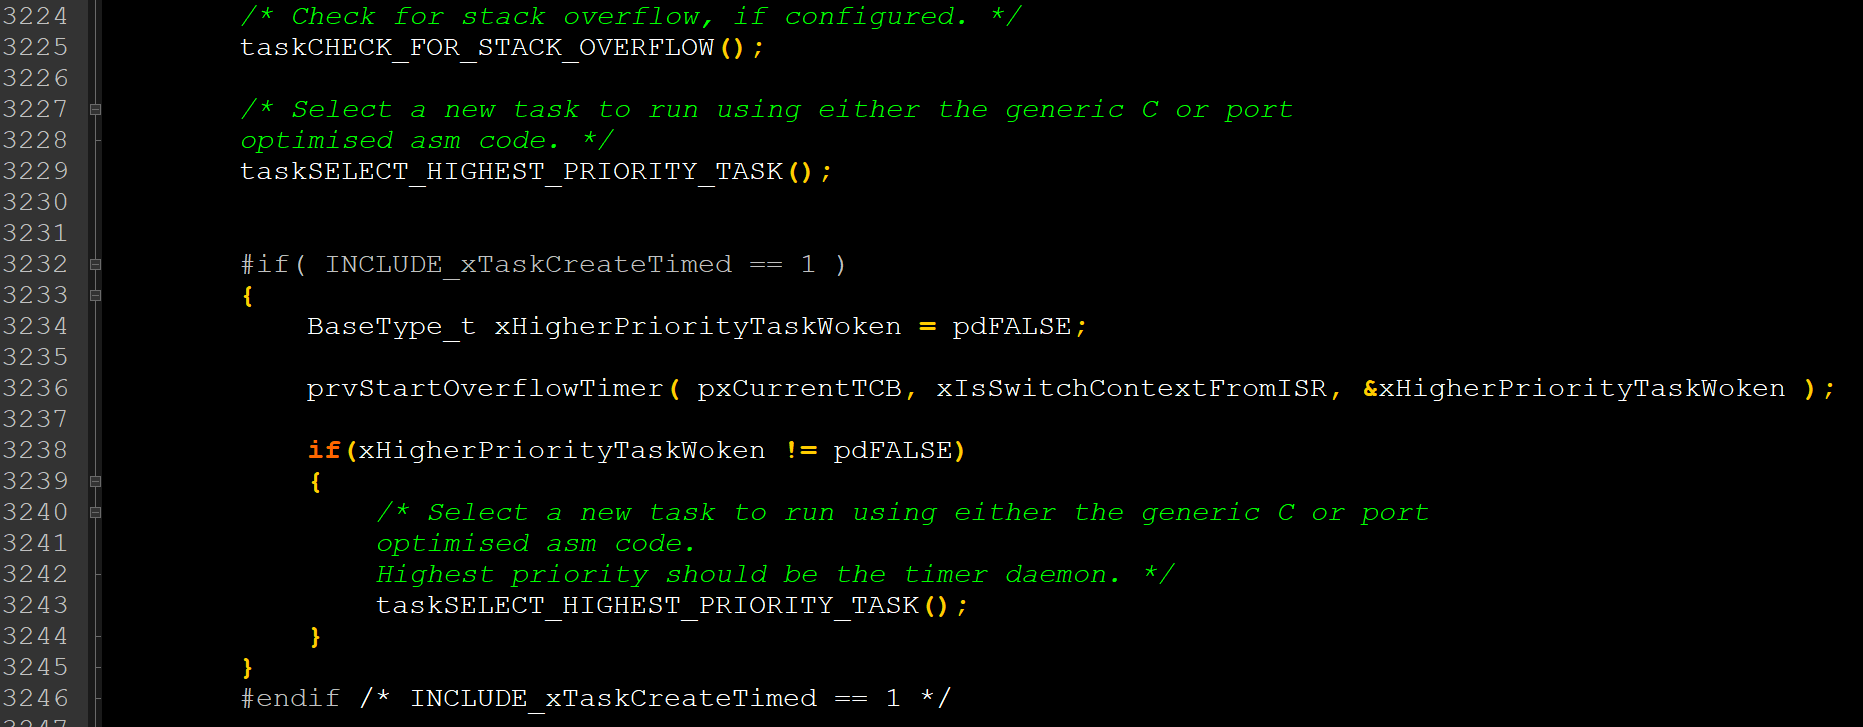
\includegraphics[width=\linewidth]{images/freertos_overflow_start.png}
      \caption{Starting of the overflow timer from the file task.c}
      \label{fig:freertos_overflow_start}
    
\end{figure}

The overrun timer is, in the beginning, just a TickType\textunderscore t variable xOverrunTicks in the task's control block. It is incremented every tick timed task is running. When it is over the maximal value it start a software timer with a timeout of 1 tick. Timer daemon triggers the overrrun callback one tick later. Code for incrementing (\autoref{fig:freertos_overrun_increment}) is called from the function xTaskIncrementTick which itself is called from the tick interrupt. Overrun timer (of period 1 tick) is started from the context switch function, with code shown in \autoref{fig:freertos_overrun_start}.

\begin{figure}[H]

      \centering
      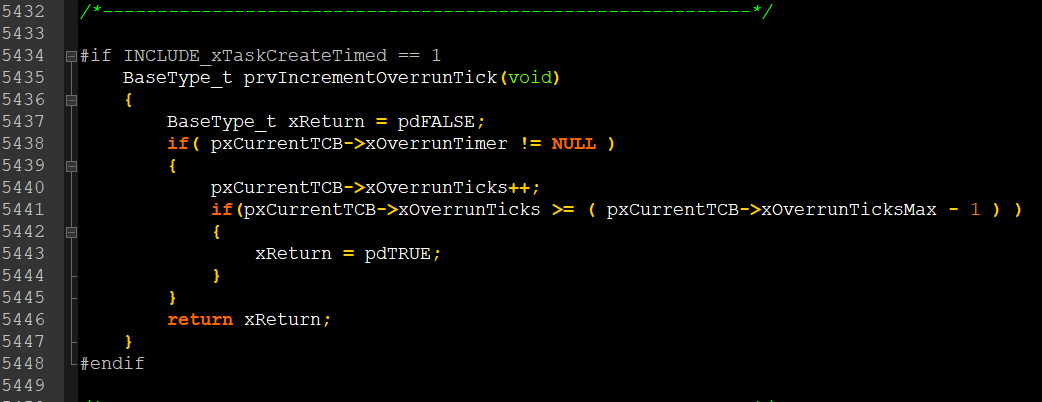
\includegraphics[width=\linewidth]{images/freertos_overrrun_increment.png}
      \caption{Incrementing of the overrun timer from the file task.c}
      \label{fig:freertos_overrun_increment}
    
\end{figure}

\begin{figure}[H]

      \centering
      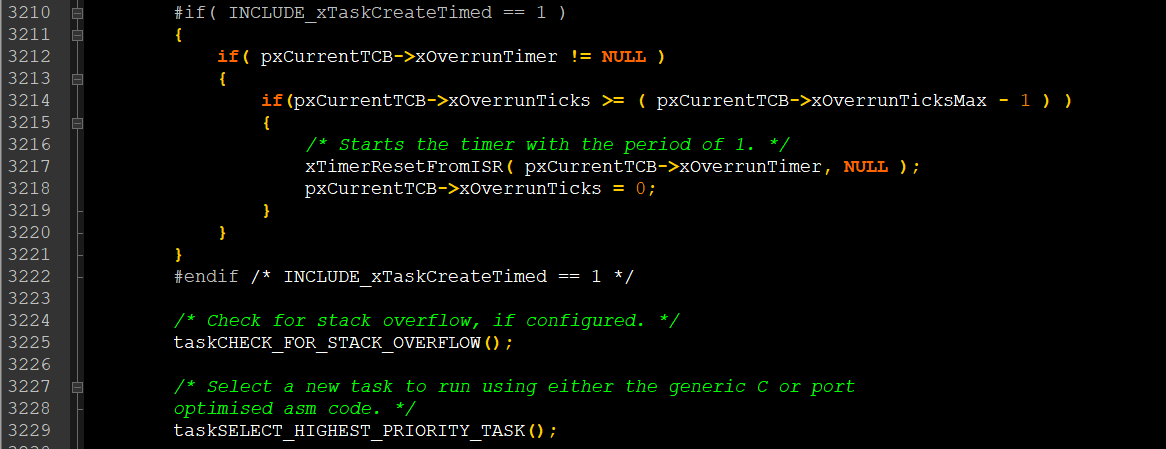
\includegraphics[width=\linewidth]{images/freertos_overrun_start.png}
      \caption{Starting of the overrun timer from the file task.c}
      \label{fig:freertos_overrun_start}
    
\end{figure}


 Next three figures showcase how the timed tasks work. \autoref{fig:timed_example_overrun} shows when is overrun timer triggered. Similarly, \autoref{fig:timed_example_overflow} showcases how the overflow timer works. Finally, \autoref{fig:timed_example_reset} shows how reseting the timed task suppresses the timeout of overflow and overrun timers.

\begin{figure}[H]

      \centering
      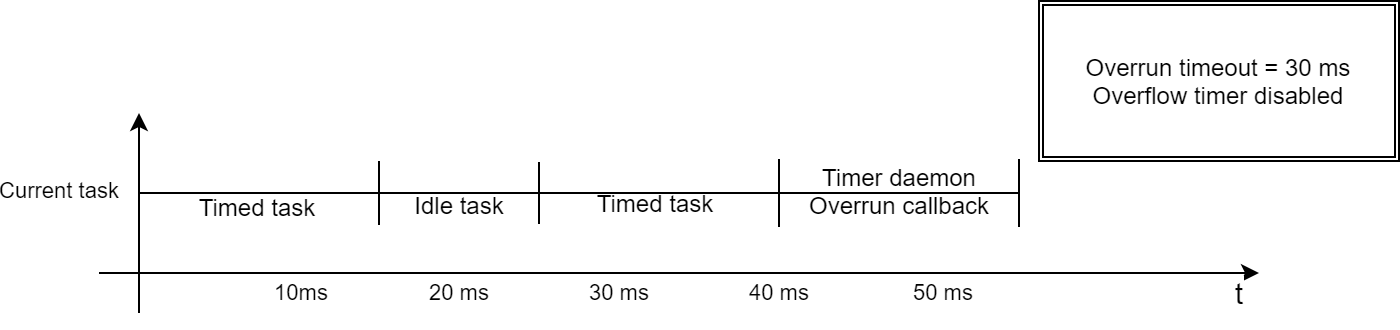
\includegraphics[width=\linewidth]{images/timed_example_overrun.png}
      \caption{Timed task with overrun timeout of 30 ms}
      \label{fig:timed_example_overrun}
    
\end{figure}

\begin{figure}[H]

      \centering
      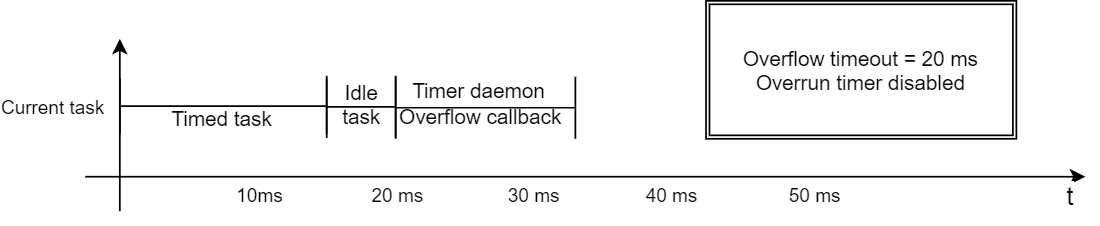
\includegraphics[width=\linewidth]{images/timed_example_overflow.png}
      \caption{Timed task with overflow timeout of 20 ms}
      \label{fig:timed_example_overflow}
    
\end{figure}

\begin{figure}[H]

      \centering
      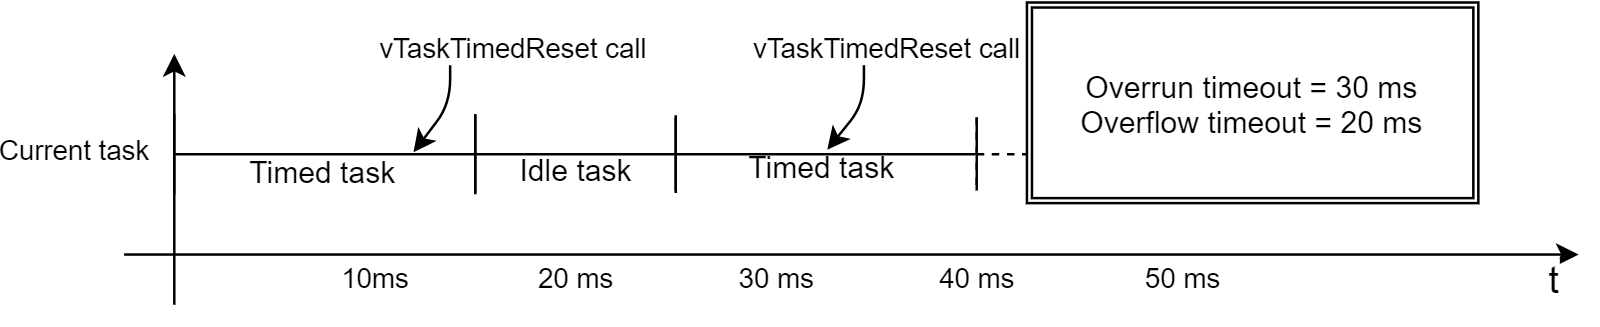
\includegraphics[width=\linewidth]{images/timed_example_reset.png}
      \caption{Timed task with both timers that resets in time}
      \label{fig:timed_example_reset}
    
\end{figure}

vTaskDelete function is changed so that deleting tasks also deletes their timers.

\subsection{Limitiations}

Static create of the function is not available.

Timer callback functions are called by the timer daemon and its priority determines when the callback will be called. It is recommended that timer deamon has the highest priority.

\section{Replicated tasks}

\subsection{Introduction}

Redundancy is a common term with safety hardware, but the redundancy can be achieved with the software. As is demonstrated with the replicated tasks. As the name suggests, when replicated tasks are created they make more parallel instances and they compare outputs of each other to assure no errors happened. 

Hardware redundancy has the advantage of detecting the fault as early as possible at the cost of increased hardware. On the other hand, software redundancy is useful when the system cost is the restriction ss no additional hardware is needed. 

\noindent Two types of replicated tasks are implemented:
\begin{itemize}
    \item 2oo2\footnote{MooN is read as M out of N. It shows how many valid outputs have to be present for valid operation e.g. 1oo2 means 1 valid output out of 2 have to be present for a valid operation} configuration or without recovery
    \item 2oo3 configuration or with recovery
\end{itemize}

Recovery of 2oo3 configuration can be achieved with voting logic. Voting logic can determine which two tasks have the same output and make it a valid one. Same is not possible with 2oo2 voting logic.


\subsection{Architecture}

Replicated tasks have an ability to detect errors using at least two tasks performing identical operations. Tasks are independently processed by the processor. Output variables from tasks are compared in real time. In case of discrepancy in the output variables, an error callback is called where user can process the error.

\autoref{fig:replicated_example} shows how replicated task with recovery works. It shows that all instances wait on the barrier. When all tasks have arrived their compare values are compared. In case of an missmatch, the callback given on task creation is called. 


\begin{figure}[H]

      \centering
      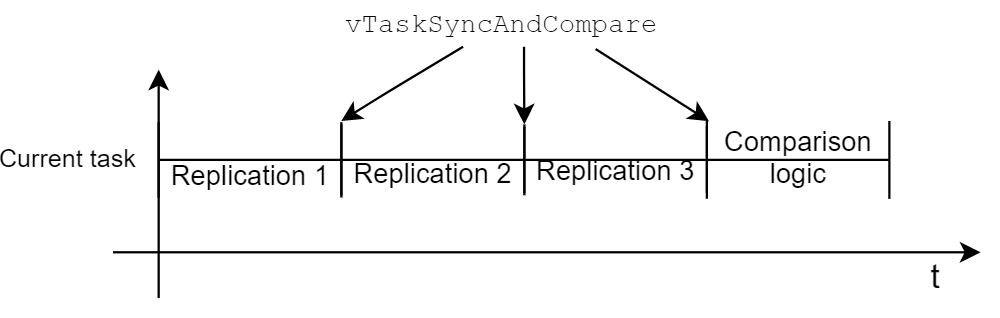
\includegraphics[width=\linewidth]{images/replicated_example.png}
      \caption{Replicated task with redundancy}
      \label{fig:replicated_example}
    
\end{figure}

Comparison logic is not a new task for itself. It is done within one of the tasks. Whichever arrives last. vTaskDelete function was modified so that when one of the replicated sub-tasks delete is requested all linked will be deleted. Tasks are linked over the TCBs\footnote{TCB - Task control block}.

\subsection{Limitiations}

Static create of the timed tasks is not available.

\section{Command reference}

Timed tasks:
\begin{itemize}

    \item \nameref{rt_cmd:xTaskCreateTimed}
    \item \nameref{rt_cmd:vTaskTimedReset}
    \item \nameref{rt_cmd:xTimerGetTaskHandle}
    
\end{itemize}

\noindent Replicated tasks:
\begin{itemize}

    \item \nameref{rt_cmd:xTaskCreateReplicated}
    \item \nameref{rt_cmd:xTaskSetCompareValue}
    \item \nameref{rt_cmd:vTaskSyncAndCompare}
    
\end{itemize}

\noindent General added functions:
\begin{itemize}

    \item \nameref{rt_cmd:eTaskGetType}
    \item \nameref{rt_cmd:xTimerPause}
    \item \nameref{rt_cmd:xTimerPauseFromISR}
    \item \nameref{rt_cmd:xTimerResume}
    \item \nameref{rt_cmd:xTimerResumeFromISR}
    \item \nameref{rt_cmd:xTimerIsTimerActiveFromISR}
    
\end{itemize}

\subsection{xTaskCreateTimed -  Creates a timed task.}
\label{rt_cmd:xTaskCreateTimed}

\begin{minted}[breaklines, linenos]{c}

BaseType_t xTaskCreateTimed( TaskFunction_t pxTaskCode,
                    const char * const pcName,
                    const configSTACK_DEPTH_TYPE usStackDepth,
                    void * const pvParameters,
                    UBaseType_t uxPriority,
                    TaskHandle_t * const pxCreatedTask,
                    TickType_t xOverrunTime,
                    WorstTimeTimerCb_t pxOverrunTimerCb,
                    TickType_t xOverflowTime,
                    WorstTimeTimerCb_t pxOverflowTimerCb )
            
\end{minted}

\begin{lstlisting}        
Create a new timed task and add it to the list of tasks that are ready to
run.

Overrun timer is synchronous with the task and its counter is incremented
only when timed task is in running state. Overrun callback is called from
timer daemon. When timed task overruns it sends a signal to the timer daemon
and when callback is called is dependent on daemon's priority. If overrun
timer is not used send 0 for xOverrunTime or NULL for the callback.

Overflow timer is asynchronous with the task and its counter is incremented
every tick regardless of the state. Callback is called from timer daemon and
its punctuality is dependent on timer daemon's priority. If overflow timer
is not used send 0 for xOverflowTime or NULL for the callback.

Internally, within the FreeRTOS implementation, tasks use two blocks of
memory.  The first block is used to hold the task's data structures.  The
second block is used by the task as its stack.  If a task is created using
xTaskCreateTimed() then both blocks of memory are automatically dynamically
allocated inside the xTaskCreate() function.  (see
http://www.freertos.org/a00111.html). Static version of the function is not
implemented.

Input paramters:
 - pvTaskCode - Pointer to the task entry function.  Tasks
must be implemented to never return (i.e. continuous loop).

- pcName - A descriptive name for the task.  This is mainly used to
facilitate debugging.  Max length defined by configMAX_TASK_NAME_LEN - default is 16.

- usStackDepth -The size of the task stack specified as the number of
variables the stack can hold - not the number of bytes.  For example, if
the stack is 16 bits wide and usStackDepth is defined as 100, 200 bytes
will be allocated for stack storage.

- pvParameters - Pointer that will be used as the parameter for the task
being created.

- uxPriority - The priority at which the task should run.  Systems that
include MPU support can optionally create tasks in a privileged (system)
mode by setting bit portPRIVILEGE_BIT of the priority parameter.  For
example, to create a privileged task at priority 2 the uxPriority parameter
should be set to ( 2 | portPRIVILEGE_BIT ).

- pvCreatedTask - Used to pass back a handle by which the created task
can be referenced.

- xOverrunTime - Runtime of the task after which callback will be called.

- pxOverrunTimerCb - Pointer to the function that will be called if task
runs longer than xOverrunTime without reseting the timed task. Overrun timer
is synchronous with the task and its tick is only incremented when timed
task is in running state.

- xOverflowTime - Asynchronous timer time. After xOverflowTime
pxOverflowTimerCb will be called.

- pxOverflowTimerCb - Pointer to the function that will be called after
xOverflowTime. Overflow timer is asynchronous from the task and its value is
incremented every tick.

Returns pdPASS if the task was successfully created and added to a ready
list, otherwise an error code defined in the file projdefs.h
Example usage:

\end{lstlisting}

\begin{minted}[breaklines, linenos]{c}
 // Task to be created.
 void vTaskTimedCode( void * pvParameters )
 {
     for( ;; )
     {
         // Task code goes here.

         // Reset the timer.
         vTaskTimedReset(NULL);
     }
 }

// Function to be called if timer overflows.
void vTaskOverflowCallback ( WorstTimeTimerHandle_t xTimer )
{
    // Timeout callback code.

    // Maybe task deletion is needed. Calling vTaskDelete automatically deletes
    // the timer too. Do NOT delete the timer directly. That will cause
    // undefined behavior when deleting the task.
    vTaskDelete( xTimerGetTaskHandle( xTimer ) );
}
// Function to be called if timer overflows.
void vTaskOverrunCallback ( WorstTimeTimerHandle_t xTimer )
{

    // Timeout callback code.

    // Maybe task deletion is needed. Calling vTaskDelete automatically deletes
    // the timer too. Do NOT delete the timer directly. That will cause
    // undefined behavior when deleting the task.
    vTaskDelete( xTimerGetTaskHandle( xTimer ) );
}

 // Function that creates a task.
 void vOtherFunction( void )
 {
 static uint8_t ucParameterToPass;
 TaskHandle_t xHandle = NULL;

     // Create the task, storing the handle.  Note that the passed parameter ucParameterToPass
     // must exist for the lifetime of the task, so in this case is declared static.  If it was just an
     // an automatic stack variable it might no longer exist, or at least have been corrupted, by the time
     // the new task attempts to access it.
     xTaskCreate( vTaskCode,
                  "NAME",
                  STACK_SIZE,
                  &ucParameterToPass,
                  tskIDLE_PRIORITY,
                  &xHandle,
                  pdMS_TO_TICKS(1 * 1000),
                  vTaskOverrunCallback,
                  pdMS_TO_TICKS(2 * 1000),
                  vTaskOverflowCallback );
     configASSERT( xHandle );

     // Use the handle to delete the task.
     if( xHandle != NULL )
     {
         vTaskDelete( xHandle );
     }
 }

\end{minted}

\subsection{vTaskTimedReset -  Resets the timer of timed task.}
\label{rt_cmd:vTaskTimedReset}


\begin{minted}[breaklines, linenos]{c}
void vTaskTimedReset( TaskHandle_t pxTaskHandle )
\end{minted}

\begin{lstlisting}
Reset the timer of the timed task.

- Warning - Shall only be used for timed tasks.

Input parameters:

- pxTaskHandle - Handle of the task whose timer shall be reset.
Passing a NULL handle results in reseting the timer of the calling task.

Example usage:
\end{lstlisting}

\begin{minted}[breaklines, linenos]{c}
void vTimedTask( void * pvParameters )
{
    for( ;; )
    {
        // Task code goes here.

        vTaskTimedReset(NULL);
    }
}
\end{minted}

\subsection{xTimerGetTaskHandle -  Gets the corresponding timed task handle from the timer handle.}
\label{rt_cmd:xTimerGetTaskHandle}
\begin{minted}[breaklines, linenos]{c}
TaskHandle_t xTimerGetTaskHandle( const TimerHandle_t xTimer )
\end{minted}
\begin{lstlisting}
Returns the timed task handle assigned to the timer. Task handle is an union
with timer ID and that is why they are mutually exclusive.

Task handle is assigned to the timer when creating the timed task.

WARNING: Setting the timer ID also sets the task handle. Changing the timer
ID can lead to undefined behavior.

Input parameters:

- xTimer - The timer being queried.

Example usage:

- See xTaskCreateTimed

\end{lstlisting}
\subsection{xTaskCreateReplicated -  Creates a replicated task.}
\label{rt_cmd:xTaskCreateReplicated}

\begin{minted}[breaklines, linenos]{c}
BaseType_t xTaskCreateReplicated( TaskFunction_t pxTaskCode,
                                  const char * const pcName,
                                  const configSTACK_DEPTH_TYPE usStackDepth,
                                  void * const pvParameters,
                                  UBaseType_t uxPriority,
                                  TaskHandle_t * const pxCreatedTask,
                                  uint8_t ucReplicatedType,
                                  RedundantValueErrorCb_t pxRedundantValueErrorCb )
\end{minted}

\begin{lstlisting}
Create a new replicated task and add it to the list of tasks that are ready
to run. Replicated task is used to achieve redundancy of the software at the
expense of slower execution. Task executes slower because it is replicated
two or three times. Depending  on the type chosen. On every call to
vTaskSyncAndCompare task is suspended until every replicated task arrives to
the same point. When every task is in the synchronization function
comparison is done. If any of the comparison results differ callback
function pxRedundantValueErrorCb is called. In the callback function
user can access the compare values and choose whether to delete all the
tasks.

Internally, within the FreeRTOS implementation, tasks use two blocks of
memory.  The first block is used to hold the task's data structures.  The
second block is used by the task as its stack.  If a task is created using
xTaskCreateReplicated() then both blocks of memory are automatically
dynamically allocated inside the xTaskCreateReplicated() function.  (see
http://www.freertos.org/a00111.html). Static version of this function is not
implemented.

Input parameters:
- pvTaskCode - Pointer to the task entry function.  Tasks
must be implemented to never return (i.e. continuous loop).

- pcName - A descriptive name for the task.  This is mainly used to
 facilitate debugging.  Max length defined by configMAX_TASK_NAME_LEN - default
 is 16.

- usStackDepth - The size of the task stack specified as the number of
variables the stack can hold - not the number of bytes.  For example, if
the stack is 16 bits wide and usStackDepth is defined as 100, 200 bytes
will be allocated for stack storage.

- pvParameters - Pointer that will be used as the parameter for the task
being created.

- uxPriority - The priority at which the task should run.  Systems that
include MPU support can optionally create tasks in a privileged (system)
mode by setting bit portPRIVILEGE_BIT of the priority parameter.  For
example, to create a privileged task at priority 2 the uxPriority parameter
should be set to ( 2 | portPRIVILEGE_BIT ).

- pvCreatedTask - Used to pass back a handle by which the created task
can be referenced.

- ucReplicatedType - Valid values: taskREPLICATED_NO_RECOVERY and
taskREPLICATED_RECOVERY. No recovery is faster as it created only two
instances, but recovery is not possible. Recovery creates three identical
tasks. Recovery is possible with 2 out of 3 logic.

- pxRedundantValueErrorCb - Function to be called when compare values do
not match. Return value determines whether calling redundant task will be
deleted.

Returns pdPASS if the task was successfully created and added to a ready
list, otherwise an error code defined in the file projdefs.h


Example usage:
\end{lstlisting}
\begin{minted}[breaklines, linenos]{c}
// Task to be created.
void vTaskCode( void * pvParameters )
{
    for( ;; )
    {
        // Task code goes here.

        vTaskSyncAndCompare(&xCompareValue);
    }
}

// NOTE: This function is called from the redundant task and not daemon.
uint8_t ucCompareErrorCb (CompareValue_t * pxCompareValues, uint8_t ucLen)
{
    // Iterate through compare values.
    for(uint8_t iii = 0; iii < ucLen; i++)
    {
        pxCompareValue[iii]
        .
        .
        .
    }

    return pdTRUE; // Signaling to delete the redundant task.
}

// Function that creates a task.
void vOtherFunction( void )
{
static uint8_t ucParameterToPass;
TaskHandle_t xHandle = NULL;

    // Create the task, storing the handle.  Note that the passed parameter ucParameterToPass
    // must exist for the lifetime of the task, so in this case is declared static.  If it was just an
    // an automatic stack variable it might no longer exist, or at least have been corrupted, by the time
    // the new task attempts to access it.
    xTaskCreateReplicated( vTaskCode, "NAME", STACK_SIZE, &ucParameterToPass, tskIDLE_PRIORITY, &xHandle, taskREPLICATED_RECOVERY, ucCompareErrorCb );
    configASSERT( xHandle );

    // Use the handle to delete the task.
    if( xHandle != NULL )
    {
        vTaskDelete( xHandle );
    }
}

\end{minted}

\subsection{xTaskSetCompareValue -  Sets a compare value for the calling task.}
\label{rt_cmd:xTaskSetCompareValue}

\begin{minted}[breaklines, linenos]{c}
void xTaskSetCompareValue( CompareValue_t xNewCompareValue )

\end{minted}
\begin{lstlisting}
Sets the compare value. Compare value is used with replicated tasks. They
are used in vTaskSyncAndCompare function for figuring if there is a
difference between the tied task executions.
Input parameters:
- xNewCompareValue - New compare value to set.

\end{lstlisting}
\subsection{vTaskSyncAndCompare -  Syncronizes the replicated tasks and compares compare values.}
\label{rt_cmd:vTaskSyncAndCompare}

\begin{minted}[breaklines, linenos]{c}
void vTaskSyncAndCompare( const CompareValue_t * const pxNewCompareValue )


\end{minted}
\begin{lstlisting}
Waits until every replicated task is finished. When every task is finished
function compares the compare values and if there is a mismatch it calls the
predefined callback.

- Warning - Shall only be used for replicated tasks.

Input parameters:

- pxNewCompareValue - Pointer of the compare value to be copied from. If
NULL is passed in, previous compare value is used.

Example usage:
\end{lstlisting}
\begin{minted}[breaklines, linenos]{c}
void vReplicatedTask( void * pvParameters )
{
    for( ;; )
    {
        // Task code goes here.

        vTaskSyncAndCompare(&xCompareValue);
    }
}

\end{minted}

\subsection{eTaskGetType -  Get the type of the task.}
\label{rt_cmd:eTaskGetType}
\begin{minted}[breaklines, linenos]{c}
eTaskType eTaskGetType( TaskHandle_t pxTaskHandle )
\end{minted}
\begin{lstlisting}
Get the type of the task.

Input parameters:

- pxTaskHandle - Handle of the task to be queried.  Passing a NULL
handle results in getting the type of calling task.

\end{lstlisting}

\subsection{xTimerPause -  Pauses the timer.}
\label{rt_cmd:xTimerPause}

\begin{minted}[breaklines, linenos]{c}
BaseType_t xTimerPause( TimerHandle_t xTimer, TickType_t xTicksToWait )
\end{minted}

\begin{lstlisting}
Timer functionality is provided by a timer service/daemon task.  Many of the
public FreeRTOS timer API functions send commands to the timer service task
through a queue called the timer command queue.  The timer command queue is
private to the kernel itself and is not directly accessible to application
code.  The length of the timer command queue is set by the
configTIMER_QUEUE_LENGTH configuration constant.

xTimerPause() pauses a timer. If timer was not running before it is ignored.
Pausing remembers how many ticks until the deadline are needed and on next
xTimerResume() timer will trigger only after the ticks set by pause.

Pausing assures timer is in stopped state.
 
- xTimer - The handle of the timer being paused.

- TicksToWait - Specifies the time, in ticks, that the calling task should
be held in the Blocked state to wait for the stop command to be successfully
sent to the timer command queue, should the queue already be full when
xTimerPause() was called.  xTicksToWait is ignored if xTimerPause() is called
before the scheduler is started.

Returns pdFAIL if the pause command could not be sent to  timer command queue
even after xTicksToWait ticks had passed.  pdPASS will be returned if the
command was successfully sent to the timer command queue.
When the command is actually processed will depend on the priority of the
timer service/daemon task relative to other tasks in the system.  The timer
service/daemon task priority is set by the configTIMER_TASK_PRIORITY
configuration constant.

\end{lstlisting}

\subsection{xTimerPauseFromISR -  Pauses the timer from interrupt service routine.}
\label{rt_cmd:xTimerPauseFromISR}
\begin{minted}[breaklines, linenos]{c}
 BaseType_t xTimerPauseFromISR( TimerHandle_t xTimer,
                                BaseType_t *pxHigherPriorityTaskWoken );
\end{minted}

\begin{lstlisting}

 A version of xTimerPause() that can be called from an interrupt service
 routine.

- xTimer  - The handle of the timer being paused.

- pxHigherPriorityTaskWoken - The timer service/daemon task spends most
of its time in the Blocked state, waiting for messages to arrive on the
timer command queue.  Calling xTimerPauseFromISR() writes a message to
the timer command queue, so has the potential to transition the timer
service/daemon task out of the Blocked state.  If calling
xTimerPauseFromISR() causes the timer service/daemon task to leave the
Blocked state, and the timer service/ daemon task has a priority equal
to or greater than the currently executing task (the task that was
interrupted), then *pxHigherPriorityTaskWoken will get set to pdTRUE
internally within the xTimerPauseFromISR() function.  If xTimerPauseFromISR()
sets this value to pdTRUE then a context switch should be performed before
the interrupt exits.

Returns pdFAIL if the pause command could not be sent to  the timer
command queue.  pdPASS will be returned if the command was successfully
sent to the timer command queue.  When the command is actually processed
will depend on the priority of the timer service/daemon task relative
to other tasks in the system.  The timer service/daemon task priority is
set by the configTIMER_TASK_PRIORITY configuration constant.

\end{lstlisting}
\subsection{xTimerResume -  Resumes the timer.}
\label{rt_cmd:xTimerResume}
\begin{minted}[breaklines, linenos]{c}
 BaseType_t xTimerResume( TimerHandle_t xTimer, TickType_t xTicksToWait )
\end{minted}
\begin{lstlisting}
Timer functionality is provided by a timer service/daemon task.  Many of the
public FreeRTOS timer API functions send commands to the timer service task
through a queue called the timer command queue.  The timer command queue is
private to the kernel itself and is not directly accessible to application
code.  The length of the timer command queue is set by the
configTIMER_QUEUE_LENGTH configuration constant.

xTimerResume() resumes a timer. If timer was not running before it acts as
xTimerStart. If timer saw stopped prior to the call with xTimerPause than it
places a deadline in daemon task from the time timer left of and not the
full period.

Resuming assures timer is in running state. If the timer is not stopped,
deleted, or reset in the mean time, the callback function associated with the
timer will get called 'n' ticks after xTimerStart() was called, where 'n' is
the time left from when last pause was called.

- xTimer - The handle of the timer being resumed.

- xTicksToWait - Specifies the time, in ticks, that the calling task should
be held in the Blocked state to wait for the resume command to be
successfully sent to the timer command queue, should the queue already be
full when xTimerResume() was called.  xTicksToWait is ignored if
xTimerResume() is called before the scheduler is started.

pdFAIL will be returned if the resume command could not be sent to
the timer command queue even after xTicksToWait ticks had passed.  pdPASS
will be returned if the command was successfully sent to the timer command
queue. When the command is actually processed will depend on the priority
of the timer service/daemon task relative to other tasks in the system.
The timer service/daemon task priority is set by the
configTIMER_TASK_PRIORITY configuration constant.
\end{lstlisting}

\subsection{xTimerResumeFromISR -  Resumes the timer from interrupt service routine.}
\label{rt_cmd:xTimerResumeFromISR}
\begin{minted}[breaklines, linenos]{c}
 BaseType_t xTimerResumeFromISR(  TimerHandle_t xTimer,
                                  BaseType_t *pxHigherPriorityTaskWoken )
\end{minted}

\begin{lstlisting}
A version of xTimerResume() that can be called from an interrupt service
routine.

- xTimer - The handle of the timer being resumed.

- pxHigherPriorityTaskWoken - The timer service/daemon task spends most
of its time in the Blocked state, waiting for messages to arrive on the
timer command queue.  Calling xTimerPauseFromISR() writes a message to
the timer command queue, so has the potential to transition the timer
service/daemon task out of the Blocked state.  If calling
xTimerPauseFromISR() causes the timer service/daemon task to leave the
Blocked state, and the timer service/ daemon task has a priority equal
to or greater than the currently executing task (the task that was
interrupted), then *pxHigherPriorityTaskWoken will get set to pdTRUE
internally within the xTimerPauseFromISR() function.  If xTimerPauseFromISR()
sets this value to pdTRUE then a context switch should be performed before
the interrupt exits.

pdFAIL will be returned if the resume command could not be sent to
the timer command queue.  pdPASS will be returned if the command was
successfully sent to the timer command queue.  When the command is actually
processed will depend on the priority of the timer service/daemon task
relative to other tasks in the system.  The timer service/daemon task
priority is set by the configTIMER_TASK_PRIORITY configuration constant.

\end{lstlisting}
\subsection{xTimerIsTimerActiveFromISR -  Checks if timer is active from interrupt service routine.}
\label{rt_cmd:xTimerIsTimerActiveFromISR}

\begin{minted}[breaklines, linenos]{c}
BaseType_t xTimerIsTimerActiveFromISR( TimerHandle_t xTimer );
\end{minted}
\begin{lstlisting}
A version of xTimerIsTimerActive() that can be called from an interrupt service
routine.

- xTimer - The handle of the timer that is to be checked.

pdFAIL will be returned if the reset command could not be sent to
the timer command queue.  pdPASS will be returned if the command was
successfully sent to the timer command queue.  When the command is actually
processed will depend on the priority of the timer service/daemon task
relative to other tasks in the system, although the timers expiry time is
relative to when xTimerResetFromISR() is actually called.  The timer service/daemon
task priority is set by the configTIMER_TASK_PRIORITY configuration constant.

\end{lstlisting}
\chapter{Secure bootloader}
\label{custom_bootloader}

\section{What is a bootloader?}

Bootloaders are usually the first pieces of code that run, they run just before the user's application e.g. an operating system. They are used to manage the memory. It is highly processor and board specific. The term “bootloader” is a shortened form of the words “bootstrap loader”. The term stems from the fact that the boot manager is the key component in starting up the computer, so it can be likened to the support of a bootstrap when putting a boot on.\citep{bootloader_intro}

\section{Developed bootloader overview}

Developed bootloader can be controlled using a command shell communication over UART. The bootloader has an ablility to load new application over UART. In addition, a number of memory management functions are added. When updating the application bootloader accepts three types: binary (.bin), Intel hex (.hex) or Morotola S-record (.srec). Transmitted new application can additionally be checksummed with SHA256 or cyclic redundancy check (CRC32).

The default STM32F407 microcontroller's bootloader doesn't allow the aforementioned functionality and that is the main motivation for writing code for this platform. \citep{stm32f407_ref_man} First version of the bootloader is developed for STM32F407-Discovery board. Bootloader code is situated in the first three sectors of microcontrollers memory, as seen in \autoref{tab:bootloader_flash}. Fourth section is used as persistent memory (not loaded on the code startup) for communication between bootloader and user's application. More about application boot record in \autoref{boot_record}. 

Bootlader is written according to the BARR:C-2018 C coding standard to minimize defects in code. \citep{barr_c}

File structure of the bootloader source code for STM32F407 is as follows:
\begin{figure}[H]
\dirtree{%
.1 /.
.2 Core - Hardware initialization code and main.c.
.2 Drivers - STM's HAL Driver.
.2 custom\textunderscore bootloader - Source code of the custom bootloader. 
.3 commands.
.4 cbl\textunderscore cmds\textunderscore etc.c/.h.
.4 cbl\textunderscore cmds\textunderscore memory.c/.h.
.4 cbl\textunderscore cmds\textunderscore opt\textunderscore bytes.c/.h.
.4 cbl\textunderscore cmds\textunderscore template.c/.h.
.4 cbl\textunderscore cmds\textunderscore update\textunderscore act.c/.h.
.4 cbl\textunderscore cmds\textunderscore update\textunderscore new.c/.h.
.3 etc.
.4 cbl\textunderscore boot\textunderscore record.c/.h.
.4 cbl\textunderscore checksum.c/.h.
.4 cbl\textunderscore common.c/.h.
.3 custom\textunderscore bootloader.c.h.
.2 custom\textunderscore bootloader\textunderscore system - HAL for the custom bootloader. 
.2 startup - Contains assembly file for start up. 
.2 third\textunderscore party.
.3 sha256 - Used for checksum when loading new file. 
}
\caption{Bootloader file structure for STM32F4007 microcontroller}
\label{tree:bootloader}
\end{figure}

\section{The bootloader's architecture}

The bootloader architecture is simple. On entry, the bootloader checks if blue button on the discovery board is pressed, if it is pressed bootloader is skipped and user's application starts. Bootloader starts otherwise. On bootloader start, it checks if user's application update is needed and updates it if needed. Next step is going into system state machine.

Bootloader has 3 states: Operation, error and exit. Operation state flow is shown in \autoref{fig:bootloader_flow}. Operation state waits for incomming commands and processes them, error state constructs and sends error message back to the user. Exit state is called right before exiting, it is used to deconstruct data from the bootloader.



\begin{figure}[H]
    \centering
    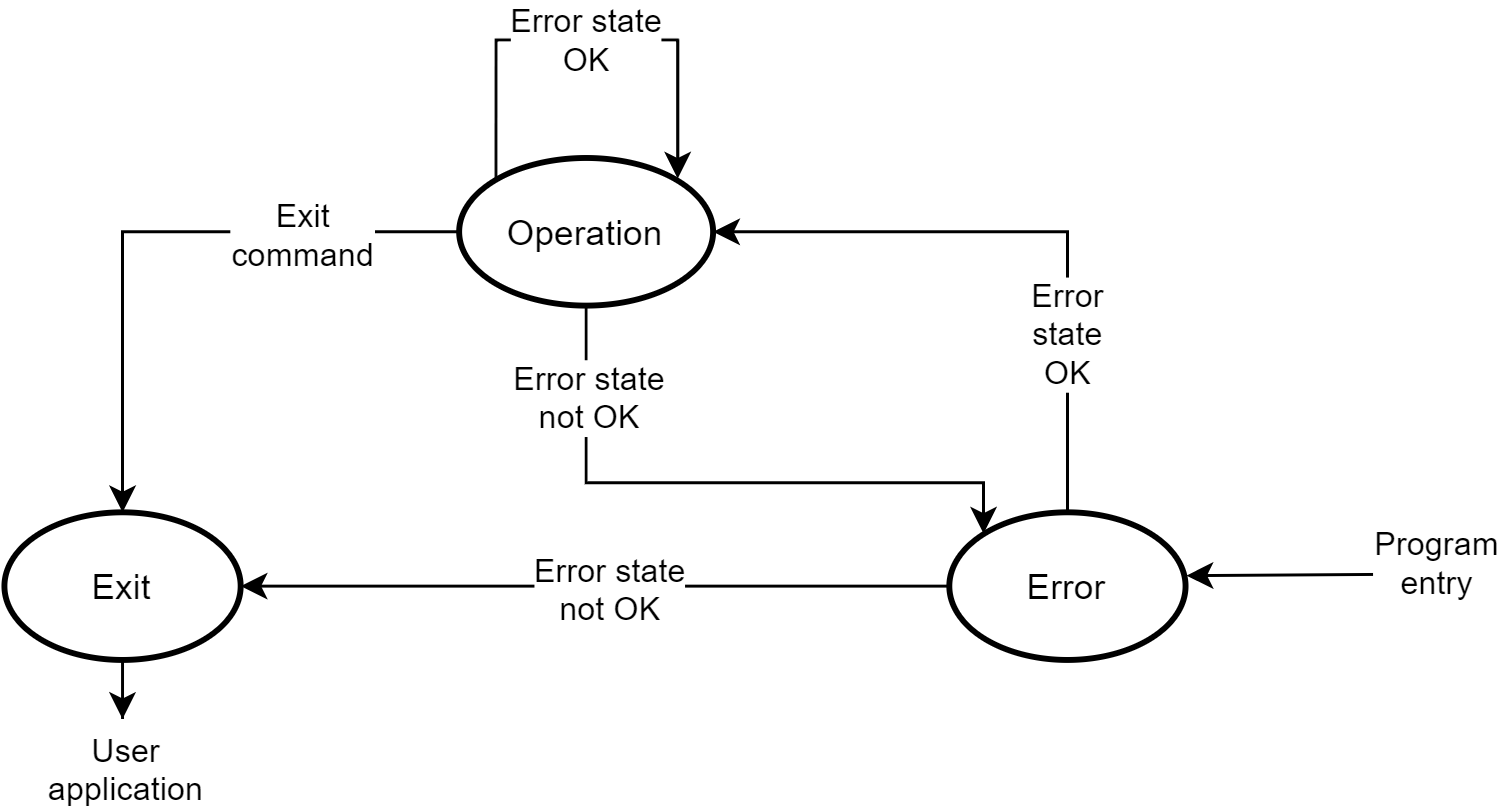
\includegraphics[width=.8\linewidth]{images/bootloader_flow.png}
    \captionof{figure}{State machine of the bootloader}
    \label{fig:bootloader_flow}
\end{figure}

\begin{figure}[H]
    \centering
    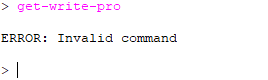
\includegraphics[width=.4\linewidth]{images/bootloader_cmd_err.png}
    \captionof{figure}{Example of an error from error state}
    \label{fig:bootloader_cmd_err}
\end{figure}

\section{Flash memory organization}

When using the bootloader the flash module is organized a shown in \autoref{tab:bootloader_flash}. 

\begin{table}[H]
\begin{tabular}{lllll}
\textbf{Block} & \textbf{Used by} & \textbf{Name} & \textbf{Block base addresses} & \textbf{Size} \\
 & \cellcolor[HTML]{D9D9D9} & \cellcolor[HTML]{D9D9D9}Sector   0 & \cellcolor[HTML]{D9D9D9}0x0800   0000 - 0x0800 3FFF & \cellcolor[HTML]{D9D9D9}16   Kbytes \\
 & \cellcolor[HTML]{D9D9D9} & \cellcolor[HTML]{D9D9D9}Sector   1 & \cellcolor[HTML]{D9D9D9}0x0800   4000 - 0x0800 7FFF & \cellcolor[HTML]{D9D9D9}16   Kbytes \\
 & \multirow{-3}{*}{\cellcolor[HTML]{D9D9D9}Bootloader} & \cellcolor[HTML]{D9D9D9}Sector   2 & \cellcolor[HTML]{D9D9D9}0x0800   8000 - 0x0800 BFFF & \cellcolor[HTML]{D9D9D9}16   Kbytes \\
 & Boot record & Sector   3 & 0x0800   C000 - 0x0800 FFFF & 16   Kbytes \\
 & \cellcolor[HTML]{D9D9D9} & \cellcolor[HTML]{D9D9D9}Sector   4 & \cellcolor[HTML]{D9D9D9}0x0801   0000 - 0x0801 FFFF & \cellcolor[HTML]{D9D9D9}64   Kbytes \\
 & \cellcolor[HTML]{D9D9D9} & \cellcolor[HTML]{D9D9D9}Sector   5 & \cellcolor[HTML]{D9D9D9}0x0802   0000 - 0x0803 FFFF & \cellcolor[HTML]{D9D9D9}128   Kbytes \\
 & \cellcolor[HTML]{D9D9D9} & \cellcolor[HTML]{D9D9D9}Sector   6 & \cellcolor[HTML]{D9D9D9}0x0804   0000 - 0x0805 FFFF & \cellcolor[HTML]{D9D9D9}128   Kbytes \\
 & \multirow{-4}{*}{\cellcolor[HTML]{D9D9D9}\begin{tabular}[c]{@{}l@{}}Current\\ application\end{tabular}} & \cellcolor[HTML]{D9D9D9}Sector   7 & \cellcolor[HTML]{D9D9D9}0x0806   0000 - 0x0807 FFFF & \cellcolor[HTML]{D9D9D9}128   Kbytes \\
 &  & Sector   8 & 0x0808   0000 - 0x0809 FFFF & 128   Kbytes \\
 &  & Sector   9 & 0x080A   0000 - 0x080B FFFF & 128   Kbytes \\
 &  & Sector   10 & 0x080C   0000 - 0x080D FFFF & 128   Kbytes \\
\multirow{-12}{*}{Main   memory} & \multirow{-4}{*}{\begin{tabular}[c]{@{}l@{}}New\\    \\ application\end{tabular}} & Sector   11 & 0x080E   0000 - 0x080F FFFF & 128   Kbytes \\
\rowcolor[HTML]{D9D9D9} 
\multicolumn{3}{l}{\cellcolor[HTML]{D9D9D9}System memory} & 0x1FFF   0000 - 0x1FFF 77FF & 30   Kbytes \\
\rowcolor[HTML]{D9D9D9} 
\multicolumn{3}{l}{\cellcolor[HTML]{D9D9D9}OTP area} & 0x1FFF   7800 - 0x1FFF 7A0F & 528   bytes \\
\rowcolor[HTML]{D9D9D9} 
\multicolumn{3}{l}{\cellcolor[HTML]{D9D9D9}Option bytes} & 0x1FFF   C000 - 0x1FFF C00F & 16   bytes
\end{tabular}
\caption{STM32F407 flash memory organization}
\label{tab:bootloader_flash}
\end{table}


\section{Application boot record}
\label{boot_record}

Aplication boot record is used to store meta data about the current user's application and new user's application. Meta data consists of: 
\begin{itemize}
    \item Checksum used for transmission,
    \item Application type used while transmitting,
    \item Length of application during transmission.
\end{itemize}
Boot record is also used to signalize that update of the application is needed to the bootloader. Flag is set when new application is successfully transmitted.

\autoref{memory_areas} and \autoref{app_boot_rec} show modifications added to the linker file needed to add the boot record. Address 0x800C000 is the starting address of sector 3 of the flash memory.

\begin{lstlisting}[frame=single, label={memory_areas}, caption={Memory areas from the linker file.}, captionpos=b]
/* Specify the memory areas */
MEMORY
{
RAM (xrw)      : ORIGIN = 0x20000000, LENGTH = 128K
CCMRAM (rw)      : ORIGIN = 0x10000000, LENGTH = 64K
/* Allow bootloader only first 3 sectors */
FLASH (rx)      : ORIGIN = 0x8000000, LENGTH = 48K 
/* Allow sector 3 for app boot record */
SEC3 (rx)		: ORIGIN = 0x800C000, LENGTH = 16K
}
\end{lstlisting}

\begin{lstlisting}[frame=single, label={app_boot_rec}, caption={Application boot record from the linker file.}, captionpos=b]
  /* Application boot record */
  .appbr 0x800C000 (NOLOAD):
  {
    . = ALIGN(4);
    _sappbr = .;       
    *(.appbr)
    *(.appbr*)
    
    . = ALIGN(4);
    _eappbr = .;   
  } >SEC3
\end{lstlisting}


\section{User application modifications}

On the start of every STM32F407 program is a vector table. Vector table contains numerous interrupt and exception vectors. List of all vectors is avaliable in \citep[p.~372]{stm32f407_ref_man}. On start up the program calls the vector on the address 4, the name of that vector is fittingly Reset handler. But before calling the reset handler main stack pointer(MSP) is set from the address 0. 

Because the program expects the main stack pointer and reset handler vector to be on the start of the program vector offset register(VTOR) is available. Vector offset register is simply added onto the flash memory base address to allow multiple programs in the same flash memory. Perfect for writing a bootloader!

To sum up, before bootloader jumps to the user application it must set the MSP to the one of the user's application then it jumps to the application's reset handler. Vector offset register can be set be the bootloader or in the user's application, former is chosen in this project.


\section{Command reference}

Important notices:

\begin{itemize}
 \item Every execute of a command must end with \textbackslash r \textbackslash n

 \item Commands are case insensitive
 
 \item On error bootloader returns "ERROR:<Explanation of error>"
 
 \item Optional parameters are surrounded with [] e.g. [example]

\end{itemize}

\noindent List of all commands:

\begin{itemize}

    \item \nameref{bl_cmd:version}
    \item \nameref{bl_cmd:help}
    \item \nameref{bl_cmd:reset}
    \item \nameref{bl_cmd:cid}
    \item \nameref{bl_cmd:get-rdp-level}
    \item \nameref{bl_cmd:jump-to}
    \item \nameref{bl_cmd:flash-erase}
    \item \nameref{bl_cmd:flash-write}
    \item \nameref{bl_cmd:mem-read}
    \item \nameref{bl_cmd:update-act} 
    \item \nameref{bl_cmd:update-new}
    \item \nameref{bl_cmd:en-write-prot}
    \item \nameref{bl_cmd:dis-write-prot}
    \item \nameref{bl_cmd:get-write-prot}
    \item \nameref{bl_cmd:exit}

\end{itemize}



\subsection{version - Gets a version of the bootloader.}
\label{bl_cmd:version}

Parameters:
\begin{lstlisting}
 - None
Execute command: 

    > version  
    
Response: 

    v1.0  
\end{lstlisting}
    
    
\subsection{help - Makes life easier.}
\label{bl_cmd:help}

\begin{lstlisting}
Parameters:

 -  None

Execute command: 

    > help  
    
Response: 

    <List of all available commands and examples>
\end{lstlisting}

\subsection{reset - Resets the microcontroller.}
\label{bl_cmd:reset}

\begin{lstlisting}
Parameters:

 - None

Execute command: 

    > reset
    
Response: 

    OK
\end{lstlisting}


\subsection{cid - Gets chip identification number.}
\label{bl_cmd:cid}

\begin{lstlisting}
Parameters:

 - None

Execute command: 

    > cid  
    
Response: 

    0x413
\end{lstlisting}

\subsection{get-rdp-level - Gets read protection \texorpdfstring{\protect\cite[p.~93]{stm32f407_ref_man}}{}}
\label{bl_cmd:get-rdp-level}

\begin{lstlisting}
Parameters:

  - None

Execute command: 

    > get-rdp-level  
    
Response: 

    level 0
\end{lstlisting}
    
\subsection{jump-to - Jumps to a requested address.}
\label{bl_cmd:jump-to}

\begin{lstlisting}
Parameters:

- addr - Address to jump to in hex format (e.g. 0x12345678), 0x can be omitted

Execute command: 

    > jump-to addr=0x87654321 
     
Response: 

    OK
\end{lstlisting}
     
\subsection{flash-erase - Erases flash memory.}
\label{bl_cmd:flash-erase}

\begin{lstlisting}
Parameters:

- type - Defines type of flash erase. "mass" erases all sectors, "sector" erases only selected sectors
    
- sector - First sector to erase. Bootloader is on sectors 0, 1 and 2. Not needed with mass erase
    
- count - Number of sectors to erase. Not needed with mass erase

Execute command: 

    > flash-erase sector=3 type=sector count=4 
     
Response: 

    OK
\end{lstlisting}

\subsection{flash-write - Writes to flash memory.}
\label{bl_cmd:flash-write}

\begin{lstlisting}
Parameters:

 - start - Starting address in hex format (e.g. 0x12345678), 0x can be omitted
     
 - count - Number of bytes to write, without checksum. Chunk size: 5120
 
 - [cksum] - Defines the checksum to use. If not present no checksum is assumed. WARNING: Even if checksum is wrong data will be written into flash memory!
 
      - "sha256" - Gives best protection (32 bytes), slowest, uses software implementation
           
      - "crc32" - Medium protection (4 bytes), fast, uses hardware implementation. Settings in [Apendix A](#apend_a)

      - "no" - No protection, fastest

Note:

  When using crc-32 checksum sent data has to be divisible by 4

Execute command: 

    > flash-write start=0x87654321 count=64 cksum=crc32  
    
Response: 

    chunks:1

    chunk:0|length:64|address:0x87654321

    ready
    
Send bytes:

    <64 bytes>
    
Response:

    chunk OK

    checksum|length:4

    ready
 
Send checksum:
     
     <4 bytes>
     
Response:
 
    OK
\end{lstlisting}

\subsection{mem-read - Read bytes from memory.}
\label{bl_cmd:mem-read}

\begin{lstlisting}
Parameters:

- start - Starting address in hex format (e.g. 0x12345678), 0x can be omitted
     
- count - Number of bytes to read

Execute command: 

    > mem-read start=0x87654321 count=3  
    
Response: 

    <3 bytes starting from the address 0x87654321>
    
Note:
- Entering invalid read address crashes the program and reboot is required. 
\end{lstlisting}

\subsection{update-act - Updates active application from new application memory area.}
\label{bl_cmd:update-act}

\begin{lstlisting}
Parameters:
- [force] - Forces update even if not needed

   - "true" - Force the update
                
   - "false" - Don't force the update


Execute command: 

    > update-act force=true
    
Response: 

    No update needed for user application
    Updating user application
    OK
\end{lstlisting}
    

\subsection{update-new - Updates new application.}
\label{bl_cmd:update-new}

\begin{lstlisting}
Parameters:

 - count - Number of bytes to write, without checksum. Chunk size: 5120
 
 - type - Type of application coding
       
      - "bin" - Binary format (.bin)
                
      - "hex" - Intel hex format (.hex)
      
      - "srec" - Motorola S-record format (.srec)
 
 - [cksum] - Defines the checksum to use. If not present no checksum is assumed. WARNING: Even if checksum is wrong data will be written into flash memory!
 
      - "sha256" - Gives best protection (32 bytes), slowest, uses software implementation
           
      - "crc32" - Medium protection (4 bytes), fast, uses hardware implementation. Settings in [Apendix A](#apend_a)

      - "no" - No protection, fastest


Execute command: 

    > update-new count=4 type=bin cksum=sha256
    
Response: 

    chunks:1

    chunk:0|length:4|address:0x08080000

    ready
    
Send bytes:

    <4 bytes>
    
Response:

    chunk OK

    checksum|length:32

    ready
 
Send checksum:
     
     <32 bytes>
     
Response:
 
    OK
\end{lstlisting}

\subsection{en-write-prot - Enables write protection per sector.}
\label{bl_cmd:en-write-prot}

\begin{lstlisting}
Parameters:

- mask - Mask in hex form for sectors where LSB corresponds to sector 0

Execute command: 

    > en-write-prot mask=0xFF0
    
Response: 

    OK
\end{lstlisting}
    
\subsection{dis-write-prot - Disables write protection per sector.}
\label{bl_cmd:dis-write-prot}

\begin{lstlisting}
Parameters:

- mask - Mask in hex form for sectors where LSB corresponds to sector 0

Execute command: 

    > dis-write-prot mask=0xFF0
    
Response: 

    OK
\end{lstlisting}

\subsection{get-write-prot - Returns bit array of sector write protection.}
\label{bl_cmd:get-write-prot}Parameters:

\begin{lstlisting}
- None

Execute command: 

    > get-write-prot
    
Response: 

    0b100000000010
\end{lstlisting}

\subsection{exit - Exits the bootloader and starts the user application.}
\label{bl_cmd:exit}

\begin{lstlisting}
Parameters:

- None

Execute command: 

    > exit  
    
Response: 

    Exiting
\end{lstlisting}

\chapter{Developed software demonstration}
\label{demonstration}

\section{Overview}

This chapter showcases how the FreeRTOS modifications and the developed secure bootloader work together. Firstly, the boot-up of the bootloader is shown. After the bootloader, the example from the FreeRTOS source code demonstrating the replicated tasks is demonstrated. Next up, microcontroller is restarted and update of the user application is requested. The process of loading a new application is showcased. Loaded new application is actually an example of the timed tasks. Finally, after the load, bootloader jumps to an example of the timed tasks from the FreeRTOS modifications.

\section{Bootloader boot-up}

On boot-up, bootloader firstly checks if the blue button is pressed on the STM32F407 DISC1 development board. If the button is not pressed, bootloader checks whether the update of the user application is needed i.e. it checks the application boot record where the meta data of the current and new applications are stored.

\autoref{fig:bootloader_bootup} shows the feedback to the user on the boot-up. Firstly the preable is printed, followed up by the \code{No update needed for user application} which is printed after the application boot record is checked. Finally, \code{>} is printed and bootloader is awaiting the user's command and the blue LED is turned on.

\begin{figure}[H]
\begin{changemargin}{1cm}{1cm}
\begin{lstlisting}[escapeinside={(*}{*)}, numbers=left, numberstyle=\tiny, stepnumber=1]
*********************************************
Custom bootloader for STM32F4 Discovery board
*********************************************
*********************************************
                     v1.1
*********************************************
               Master's thesis
                  Dino Saric
            University of Zagreb
                     2020
*********************************************
          If confused type "help"          
*********************************************
No update needed for user application

OK

>
\end{lstlisting}  
\end{changemargin}
\caption{Bootloader boot-up when no update is needed}
\label{fig:bootloader_bootup}
\end{figure}

\autoref{fig:bootloader_version} showcases the version command of the bootloader.

\begin{figure}[H]
\begin{changemargin}{1cm}{1cm}
\begin{lstlisting}[escapeinside={(*}{*)}, numbers=left, numberstyle=\tiny, stepnumber=1]
> (*\color{orange}{version}*)
v1.1

OK

>  
\end{lstlisting}  
\end{changemargin}
\caption{Bootloader version command}
\label{fig:bootloader_version}
\end{figure}

\section{Replicated tasks example}

This example is run by setting the \code{EXAMPLE\textunderscore REPLICATED} in \code{FreeRTOS\textunderscore demonstration/\\example/Inc/example.h} on line 20 to 1 and disabling timed and default example. Source code that will make the demonstration easier to follow is located in \\\code{FreeRTOS\textunderscore modification/example/src/example\textunderscore replicated.c}. In the demonstration four replicated tasks are present. All of them with different configuration. \autoref{tab:replicated_task_list} lists all tasks in the demonstration.

\begin{table}[H]
\centering
\resizebox{0.7\textwidth}{!}{%
\begin{tabular}{|c|c|c|}
\hline
Task name & \begin{tabular}[c]{@{}c@{}}Replicated recovery\\ (number of sub-tasks)\end{tabular} & \begin{tabular}[c]{@{}c@{}}Always same\\ compare values\end{tabular} \\ \hline
Repl recov ok       & true (3)  & true  \\
Repl recov fail     & true (3)  & false \\
Repl non-recov ok   & false (2) & true  \\
Repl non-recov fail & false (2) & false \\ \hline
\end{tabular}%
}
\caption{All replicated tasks in demonstration}
\label{tab:replicated_task_list}
\end{table}

\autoref{fig:replicated_tasks_example_print} shows the first 11 seconds of the replicated tasks example. Number before the \code{':'} is time elapsed from the FreeRTOS start. First, task \code{Repl recov ok} arrives to the \code{vTaskSyncAndCompare}. There are three print-outs because three sub-tasks exist and are going over the same code. When the last sub-tasks arrives to the \code{vTaskSyncAndCompare} all tasks are compared. Their value matches and no callback is called, rather the tasks are unblocked and enter the 5 second delay.

Line 6, which is printed after 2 seconds of execution, shows \code{Repl non-recov ok} task which enters the sync and compare function. After the comparison both sub tasks resume, as their compare values match. On line 8, aforementioned \code{Repl recov ok} again arrives to the compare point where it is again compared. Its compare value matches and the task is resumed.

After 6 seconds, task \code{Repl recov fail} arrives to the compare point. After all three tasks have arrived they are compared. Comparison shows that not all compare values match. Two values are 0, but one is a 1. Next line shows that the software successfully deduced with voting logic that the correct result is 0 (line 16).

Right after the task \code{Repl recov fail} is done, task \code{Repl non-recov fail} arrives at the compare point. Like the last task before, the compare values don't match (line 20). The difference is that no result could be deduced this time as there are only two sub-tasks.

After the last task is finished, task \code{Repl non-recov ok} again comes to the compare function and the logic is repeated. All tasks are periodic with period of 5.

\begin{figure}[H]
\begin{changemargin}{1cm}{1cm}
\begin{lstlisting}[escapeinside={(*}{*)}, numbers=left, numberstyle=\tiny, stepnumber=1]
Jumping to user application :)
FreeRTOS Modification.
0:Task "Repl recov ok" is waiting for comparison.
4:Task "Repl recov ok" is waiting for comparison.
9:Task "Repl recov ok" is waiting for comparison.
2001:Task "Repl non-recov ok" is waiting for comparison.
2006:Task "Repl non-recov ok" is waiting for comparison.
5014:Task "Repl recov ok" is waiting for comparison.
5019:Task "Repl recov ok" is waiting for comparison.
5024:Task "Repl recov ok" is waiting for comparison.
6027:Task "Repl recov fail" is waiting for comparison.
6032:Task "Repl recov fail" is waiting for comparison.
6037:Task "Repl recov fail" is waiting for comparison.
6042:Task "Repl recov fail" compare failed.
6047:Compare values are: 0 0 1 
6050:Deduced result is 0.
6052:Task "Repl non-recov fail" is waiting for comparison.
6058:Task "Repl non-recov fail" is waiting for comparison.
6063:Task "Repl non-recov fail" compare failed.
6068:Compare values are: 0 1 
6071:Result could not be deduced.
7011:Task "Repl non-recov ok" is waiting for comparison.
7016:Task "Repl non-recov ok" is waiting for comparison.
10029:Task "Repl recov ok" is waiting for comparison.
10034:Task "Repl recov ok" is waiting for comparison.
10039:Task "Repl recov ok" is waiting for comparison.
11053:Task "Repl recov fail" is waiting for comparison.
11058:Task "Repl recov fail" is waiting for comparison.
11063:Task "Repl recov fail" is waiting for comparison.
11069:Task "Repl recov fail" compare failed.
11073:Compare values are: 1 1 0 
11076:Deduced result is 1.
\end{lstlisting}  
\end{changemargin}
\caption{Replicated tasks example output}
\label{fig:replicated_tasks_example_print}
\end{figure}

\section{New application loading}

\autoref{fig:new_application_loading} demonstrates the application flow when the user requests a user application update. To update the application user enters the function \code{update-new}, more about the function at its reference \autoref{bl_cmd:update-new}. Line 1 shows an erroneous call of the function, bootloader returns a descriptive error to the user. After the second call, all the required parameters are entered correctly. Device erases the chunks that are needed by the application, turning the blue LED signalizing that flash is being deleted.

After erasing, bootloader returns the total number of chunks the file will need to be split into. Following, on line 9, chunk 0 information is printed. Finally, \code{ready} is printed, signalizing the bootloader is ready to receive 5120 bytes. While writing the data sent by the user, the blue LED is turned on emphasizing that the flash memory is being written into. After the data is transmitted bootloader returns \code{chunk OK} to signalize that the sent bytes were successfully written into flash. The procedure is repeated for the rest of the chunks.  

When all the chunks have been written  into flash, if the checksum was specified in the function call,  it is awaited by the bootloader. This process is seen on the line 12. When the 32 bytes have been entered, inputted and calculated checksums are compared and \code{OK} is printed.

After the successful checksum, the microcontroller is automatically restarted. On the restart, it works out that the user application needs an update and it updates the user application by copying the bytes from new application (as described in \autoref{tab:bootloader_flash}) into the current application flash area.

\begin{figure}[H]
\begin{changemargin}{1cm}{1cm}
\begin{lstlisting}[escapeinside={(*}{*)}, numbers=left, numberstyle=\tiny, stepnumber=1]
> (*\color{orange}{update-new count=757720 type=hex cksum=sha256}*)
ERROR: New app is too long. Aborting
> (*\color{orange}{update-new count=75772 type=hex cksum=sha256}*)
chunks:15
chunk:0|length:5120|address:0x08080000
ready
chunk OK
(*\color{orange}{<chunks 1 - 13>}*)
chunk:14|length:4092|address:0x08091800
ready
chunk OK
checksum|length:32
ready
(*\color{orange}{<32 checksum bytes>}*)
OK
Restarting...
*********************************************
Custom bootloader for STM32F4 Discovery board
*********************************************
*********************************************
                     v1.1
*********************************************
               Master's thesis
                  Dino Saric
            University of Zagreb
                     2020
*********************************************
          If confused type "help"          
*********************************************
Update for user application available
Updating user application
OK
> 
\end{lstlisting}  
\end{changemargin}
\caption{New application loading output}
\label{fig:new_application_loading}
\end{figure}

\section{Timed tasks example}

After the successful update of the user application, timed task example is loaded into the flash. Timed example demonstrates how overrun and overflow timer work. Overrun timer increments only when the timed task is active. Overflow timer increments asynchronously to the task, i.e. it increments regardless if the timed task is active. 

\autoref{fig:timed_tasks_example_print} shows how the first 30 seconds of the example from \code{FreeRTOS\textunderscore modification/\\example/src/example\textunderscore timed.c}. The matching output is achieved by setting the \code{EXAMPLE\textunderscore TIMED} to 1 on line 19 in \code{FreeRTOS\textunderscore demonstration/example/Inc/example.h}. \autoref{tab:timed_task_list} shows all the tasks in the example.

\begin{table}[H]
\centering
\resizebox{0.8\textwidth}{!}{%
\begin{tabular}{|c|c|c|c|c|}
\hline
Task name &
  \begin{tabular}[c]{@{}c@{}}Overflow\\ timeout (s)\end{tabular} &
  \begin{tabular}[c]{@{}c@{}}Overrun\\ timeout (s)\end{tabular} &
  \begin{tabular}[c]{@{}c@{}}Period\\ (ms)\end{tabular} &
  \begin{tabular}[c]{@{}c@{}}Priority, higher is\\ more important\end{tabular} \\ \hline
Oflow task ok              & 6 & - & 5900 & 3 \\
Oflow task fail            & 6 & - & -    & 2 \\
Oflow task fail and del    & 6 & - & -    & 3 \\
Orun task ok               & - & 5 & 4900 & 3 \\
Orun task fail             & - & 5 & -    & 2 \\
Orun task fail and dele    & - & 5 & -    & 3 \\ \hline
\end{tabular}%
}
\caption{All timed tasks in demonstration}
\label{tab:timed_task_list}
\end{table}

In \autoref{fig:timed_tasks_example_print}, first task that resets the timers using the function \code{vTaskTimedReset} is the \code{Orun task ok}, it resets the timers before the overflow timer triggers so no callback is called. Next task that resets its timers is \code{Oflow task ok}, it also resets the timers before the overrun timer triggers and the callback is not called. On line 10, overflow timer from task \code{Oflow task fail and del} overflows and it deletes itself from the callback. Right after, overflow timer from task \code{Oflow task fail} triggers.

On line 12, first overrun timer is triggered. The callback deletes the task after it has been triggered. This trigger is made possible using the \code{HAL\textunderscore Delay()} function inside the task with timeout larger than the overrun timeout. On line 16, the overrun timer of the task \code{Orun task fail} triggers. Signalizing that the task was in running state for 5 seconds, during which overrun timer was not reset.

\begin{figure}[H]
\begin{changemargin}{1cm}{1cm}
\begin{lstlisting}[escapeinside={(*}{*)}, numbers=left, numberstyle=\tiny, stepnumber=1]
> (*\color{orange}{exit}*)

OK
Exiting

Jumping to user application :)
FreeRTOS Modification.
4900:Task "Orun task ok" is reseting the timer.
5900:Task "Oflow task ok" is reseting the timer.
6000:Task "Oflow task fail and del" overflowed. Deleting task.
6006:Task "Oflow task fail" overflowed. This happens every 6 s.
8120:Task "Orun task fail and dele" overran. Deleting task.
9808:Task "Orun task ok" is reseting the timer.
11809:Task "Oflow task ok" is reseting the timer.
12000:Task "Oflow task fail" overflowed. This happens every 6 s.
12239:Task "Orun task fail" overran. This happens after 5 s of runtime.
14712:Task "Orun task ok" is reseting the timer.
17713:Task "Oflow task ok" is reseting the timer.
18000:Task "Oflow task fail" overflowed. This happens every 6 s.
18258:Task "Orun task fail" overran. This happens after 5 s of runtime.
\end{lstlisting}  
\end{changemargin}
\caption{Timed tasks example output}
\label{fig:timed_tasks_example_print}
\end{figure}
\chapter{Conclusion}

This thesis explores the functional safety practices in embedded systems. Overview of functional safety and related standards is provided to help engineers without functional safety experience. The thesis clarifies how ARM Cortex R improves functional safety principles over ARM Cortex M. 

A software is developed to achieve software redundancy in ARM Cortex M. Implemented software includes a bootloader and a modified FreeRTOS operating system.  The bootloader has the ability to load new applications and other memory manipulation related operations. The bootloader also supports permanent memory for communication between bootloader and the current application. To aid security for loading of a  new application support for HEX and SREC format is provided, along with additional checksum appended to the data.

The modified FreeRTOS operating system provides features of tracking the individual tasks execution time and task replication. Tasks tracking their time have two timers, one for overrun and one for overflow. Overrun timers count only when task is active. Overflow timer always counts regardless of the task's state. Replicated tasks can have two or three redundant tasks, when three tasks are used replicated task is fault tolerant. Demonstratration of the functionality is available through examples in source code. Inner workings of FreeRTOS and the bootloader is provided in this thesis.

\bibliography{../literatura}
\bibliographystyle{../fer}

\begin{abstract}

In this thesis, an overview of functional safety and relevant standards for system development was presented. Particular emphasis was on the functional safety in embedded systems. The ARM Cortex-R architecture mechanisms for functional safety improvements over the ARM Cortex-M architecture were described. Software for redundancy implementation on an ARM Cortex-M microcontroller was developed. The software encompasses a custom-developed bootloader and a modified FreeRTOS operating system. The bootloader allows the loading of new applications and a command shell with accompanying functions. The modified FreeRTOS operating system includes the capability of tracking individual tasks execution time and the ability to replicate tasks. The implemented software functionality was demonstrated in examples.  % Gramarly OK

\keywords{Functional safety, IEC 61508, IEC 26262, bootloader, certification, ARM, Cortex R, FreeRTOS, Cortex M, kernel, redudancy, lock-step} % Gramarly OK
\end{abstract}

\hrtitle{Programska i sklopovska arhitektura redundantnih ugradbenih računalnih sustava}
\begin{sazetak}

U radu je prikazan pregled problematike funkcijske sigurnosti te su ukratko opisani odgovarajući standardi razvoja funkcijsko sigurnih sustava. Posebna pažnja posvećena je funkcijskoj sigurnosti u ugradbenim računalnim sustavima. Opisani su mehanizmi kojima ARM Cortex-R arhitektura unapređuje funkcijsku sigurnost u odnosu na ARM Cortex-M arhitekturu. Razvijena je programska potpora za ostvarivanje redundancije na mikrokontroleru s ARM Cortex-M arhitekturom. Programska potpora sadržava vlastito razvijeni bootloader i modificirani operacijski sustav FreeRTOS. Bootloader omogućuje učitavanje novih aplikacija i naredbenu ljusku s odgovarajućim funkcijama. Modificirani operacijski sustav FreeRTOS ima mogućnost praćenja vremena izvođenja pojedinih zadataka i sposobnost repliciranja zadataka (engl. task replication). Implementirana funkcionalnost je demonstrirana u primjerima.

\kljucnerijeci{Funkcijska sigurnost, IEC 61508, IEC 26262, bootloader, certifikacija, ARM, Cortex R, FreeRTOS, Cortex M, jezgra, redundancija, repliciranje zadataka}
\end{sazetak}

\begin{appendices}
\chapter{FreeRTOS redudancy API command reference} % Grammarly OK
\label{appendix_cmd_ref_freertos}

Timed tasks:
\begin{itemize}

    \item \nameref{rt_cmd:xTaskCreateTimed}
    \item \nameref{rt_cmd:vTaskTimedReset}
    \item \nameref{rt_cmd:xTimerGetTaskHandle}
    
\end{itemize}

\noindent Replicated tasks:
\begin{itemize}

    \item \nameref{rt_cmd:xTaskCreateReplicated}
    \item \nameref{rt_cmd:xTaskSetCompareValue}
    \item \nameref{rt_cmd:vTaskSyncAndCompare}
    
\end{itemize}

\noindent General added functions:
\begin{itemize}

    \item \nameref{rt_cmd:eTaskGetType}
    \item \nameref{rt_cmd:xTimerPause}
    \item \nameref{rt_cmd:xTimerPauseFromISR}
    \item \nameref{rt_cmd:xTimerResume}
    \item \nameref{rt_cmd:xTimerResumeFromISR}
    \item \nameref{rt_cmd:xTimerIsTimerActiveFromISR}
    
\end{itemize}
\pagebreak
\section{xTaskCreateTimed -  Creates a timed task.}
\label{rt_cmd:xTaskCreateTimed}

\begin{minted}[breaklines, linenos]{c}

BaseType_t xTaskCreateTimed( TaskFunction_t pxTaskCode,
                    const char * const pcName,
                    const configSTACK_DEPTH_TYPE usStackDepth,
                    void * const pvParameters,
                    UBaseType_t uxPriority,
                    TaskHandle_t * const pxCreatedTask,
                    TickType_t xOverrunTime,
                    WorstTimeTimerCb_t pxOverrunTimerCb,
                    TickType_t xOverflowTime,
                    WorstTimeTimerCb_t pxOverflowTimerCb )
            
\end{minted}

\begin{lstlisting}        
Create a new timed task and add it to the list of tasks that are ready to
run.

Overrun timer is synchronous with the task and its counter is incremented
only when timed task is in running state. Overrun callback is called from
timer daemon. When timed task overruns it sends a signal to the timer daemon
and when callback is called is dependent on daemon's priority. If overrun
timer is not used send 0 for xOverrunTime or NULL for the callback.

Overflow timer is asynchronous with the task and its counter is incremented
every tick regardless of the state. Callback is called from timer daemon and
its punctuality is dependent on timer daemon's priority. If overflow timer
is not used send 0 for xOverflowTime or NULL for the callback.

Internally, within the FreeRTOS implementation, tasks use two blocks of
memory.  The first block is used to hold the task's data structures.  The
second block is used by the task as its stack.  If a task is created using
xTaskCreateTimed() then both blocks of memory are automatically dynamically
allocated inside the xTaskCreate() function.  (see
http://www.freertos.org/a00111.html). Static version of the function is not
implemented.

Input paramters:
 - pvTaskCode - Pointer to the task entry function.  Tasks
must be implemented to never return (i.e. continuous loop).

- pcName - A descriptive name for the task.  This is mainly used to
facilitate debugging.  Max length defined by configMAX_TASK_NAME_LEN - default is 16.

- usStackDepth -The size of the task stack specified as the number of
variables the stack can hold - not the number of bytes.  For example, if
the stack is 16 bits wide and usStackDepth is defined as 100, 200 bytes
will be allocated for stack storage.

- pvParameters - Pointer that will be used as the parameter for the task
being created.

- uxPriority - The priority at which the task should run.  Systems that
include MPU support can optionally create tasks in a privileged (system)
mode by setting bit portPRIVILEGE_BIT of the priority parameter.  For
example, to create a privileged task at priority 2 the uxPriority parameter
should be set to ( 2 | portPRIVILEGE_BIT ).

- pvCreatedTask - Used to pass back a handle by which the created task
can be referenced.

- xOverrunTime - Runtime of the task after which callback will be called.

- pxOverrunTimerCb - Pointer to the function that will be called if task
runs longer than xOverrunTime without reseting the timed task. Overrun timer
is synchronous with the task and its tick is only incremented when timed
task is in running state.

- xOverflowTime - Asynchronous timer time. After xOverflowTime
pxOverflowTimerCb will be called.

- pxOverflowTimerCb - Pointer to the function that will be called after
xOverflowTime. Overflow timer is asynchronous from the task and its value is
incremented every tick.

Returns pdPASS if the task was successfully created and added to a ready
list, otherwise an error code defined in the file projdefs.h
Example usage:

\end{lstlisting}

\begin{minted}[breaklines, linenos]{c}
 // Task to be created.
 void vTaskTimedCode( void * pvParameters )
 {
     for( ;; )
     {
         // Task code goes here.

         // Reset the timer.
         vTaskTimedReset(NULL);
     }
 }

// Function to be called if timer overflows.
void vTaskOverflowCallback ( WorstTimeTimerHandle_t xTimer )
{
    // Timeout callback code.

    // Maybe task deletion is needed. Calling vTaskDelete automatically deletes
    // the timer too. Do NOT delete the timer directly. That will cause
    // undefined behavior when deleting the task.
    vTaskDelete( xTimerGetTaskHandle( xTimer ) );
}
// Function to be called if timer overflows.
void vTaskOverrunCallback ( WorstTimeTimerHandle_t xTimer )
{

    // Timeout callback code.

    // Maybe task deletion is needed. Calling vTaskDelete automatically deletes
    // the timer too. Do NOT delete the timer directly. That will cause
    // undefined behavior when deleting the task.
    vTaskDelete( xTimerGetTaskHandle( xTimer ) );
}

 // Function that creates a task.
 void vOtherFunction( void )
 {
 static uint8_t ucParameterToPass;
 TaskHandle_t xHandle = NULL;

     // Create the task, storing the handle.  Note that the passed parameter ucParameterToPass
     // must exist for the lifetime of the task, so in this case is declared static.  If it was just an
     // an automatic stack variable it might no longer exist, or at least have been corrupted, by the time
     // the new task attempts to access it.
     xTaskCreate( vTaskCode,
                  "NAME",
                  STACK_SIZE,
                  &ucParameterToPass,
                  tskIDLE_PRIORITY,
                  &xHandle,
                  pdMS_TO_TICKS(1 * 1000),
                  vTaskOverrunCallback,
                  pdMS_TO_TICKS(2 * 1000),
                  vTaskOverflowCallback );
     configASSERT( xHandle );

     // Use the handle to delete the task.
     if( xHandle != NULL )
     {
         vTaskDelete( xHandle );
     }
 }

\end{minted}

\section{vTaskTimedReset -  Resets the timer of timed task.}
\label{rt_cmd:vTaskTimedReset}


\begin{minted}[breaklines, linenos]{c}
void vTaskTimedReset( TaskHandle_t pxTaskHandle )
\end{minted}

\begin{lstlisting}
Reset the timer of the timed task.

- Warning - Shall only be used for timed tasks.

Input parameters:

- pxTaskHandle - Handle of the task whose timer shall be reset.
Passing a NULL handle results in reseting the timer of the calling task.

Example usage:
\end{lstlisting}

\begin{minted}[breaklines, linenos]{c}
void vTimedTask( void * pvParameters )
{
    for( ;; )
    {
        // Task code goes here.

        vTaskTimedReset(NULL);
    }
}
\end{minted}

\section{xTimerGetTaskHandle -  Gets the corresponding timed task handle from the timer handle.}
\label{rt_cmd:xTimerGetTaskHandle}
\begin{minted}[breaklines, linenos]{c}
TaskHandle_t xTimerGetTaskHandle( const TimerHandle_t xTimer )
\end{minted}
\begin{lstlisting}
Returns the timed task handle assigned to the timer. Task handle is an union
with timer ID and that is why they are mutually exclusive.

Task handle is assigned to the timer when creating the timed task.

WARNING: Setting the timer ID also sets the task handle. Changing the timer
ID can lead to undefined behavior.

Input parameters:

- xTimer - The timer being queried.

Example usage:

- See xTaskCreateTimed

\end{lstlisting}
\section{xTaskCreateReplicated -  Creates a replicated task.}
\label{rt_cmd:xTaskCreateReplicated}

\begin{minted}[breaklines, linenos]{c}
BaseType_t xTaskCreateReplicated( TaskFunction_t pxTaskCode,
                                  const char * const pcName,
                                  const configSTACK_DEPTH_TYPE usStackDepth,
                                  void * const pvParameters,
                                  UBaseType_t uxPriority,
                                  TaskHandle_t * const pxCreatedTask,
                                  uint8_t ucReplicatedType,
                                  RedundantValueErrorCb_t pxRedundantValueErrorCb )
\end{minted}

\begin{lstlisting}
Create a new replicated task and add it to the list of tasks that are ready
to run. Replicated task is used to achieve redundancy of the software at the
expense of slower execution. Task executes slower because it is replicated
two or three times. Depending  on the type chosen. On every call to
vTaskSyncAndCompare task is suspended until every replicated task arrives to
the same point. When every task is in the synchronization function
comparison is done. If any of the comparison results differ callback
function pxRedundantValueErrorCb is called. In the callback function
user can access the compare values and choose whether to delete all the
tasks.

Internally, within the FreeRTOS implementation, tasks use two blocks of
memory.  The first block is used to hold the task's data structures.  The
second block is used by the task as its stack.  If a task is created using
xTaskCreateReplicated() then both blocks of memory are automatically
dynamically allocated inside the xTaskCreateReplicated() function.  (see
http://www.freertos.org/a00111.html). Static version of this function is not
implemented.

Input parameters:
- pvTaskCode - Pointer to the task entry function.  Tasks
must be implemented to never return (i.e. continuous loop).

- pcName - A descriptive name for the task.  This is mainly used to
 facilitate debugging.  Max length defined by configMAX_TASK_NAME_LEN - default
 is 16.

- usStackDepth - The size of the task stack specified as the number of
variables the stack can hold - not the number of bytes.  For example, if
the stack is 16 bits wide and usStackDepth is defined as 100, 200 bytes
will be allocated for stack storage.

- pvParameters - Pointer that will be used as the parameter for the task
being created.

- uxPriority - The priority at which the task should run.  Systems that
include MPU support can optionally create tasks in a privileged (system)
mode by setting bit portPRIVILEGE_BIT of the priority parameter.  For
example, to create a privileged task at priority 2 the uxPriority parameter
should be set to ( 2 | portPRIVILEGE_BIT ).

- pvCreatedTask - Used to pass back a handle by which the created task
can be referenced.

- ucReplicatedType - Valid values: taskREPLICATED_NO_RECOVERY and
taskREPLICATED_RECOVERY. No recovery is faster as it created only two
instances, but recovery is not possible. Recovery creates three identical
tasks. Recovery is possible with 2 out of 3 logic.

- pxRedundantValueErrorCb - Function to be called when compare values do
not match. Return value determines whether calling redundant task will be
deleted.

Returns pdPASS if the task was successfully created and added to a ready
list, otherwise an error code defined in the file projdefs.h


Example usage:
\end{lstlisting}
\begin{minted}[breaklines, linenos]{c}
// Task to be created.
void vTaskCode( void * pvParameters )
{
    for( ;; )
    {
        // Task code goes here.

        vTaskSyncAndCompare(&xCompareValue);
    }
}

// NOTE: This function is called from the redundant task and not daemon.
uint8_t ucCompareErrorCb (CompareValue_t * pxCompareValues, uint8_t ucLen)
{
    // Iterate through compare values.
    for(uint8_t iii = 0; iii < ucLen; i++)
    {
        pxCompareValue[iii]
        .
        .
        .
    }

    return pdTRUE; // Signaling to delete the redundant task.
}

// Function that creates a task.
void vOtherFunction( void )
{
static uint8_t ucParameterToPass;
TaskHandle_t xHandle = NULL;

    // Create the task, storing the handle.  Note that the passed parameter ucParameterToPass
    // must exist for the lifetime of the task, so in this case is declared static.  If it was just an
    // an automatic stack variable it might no longer exist, or at least have been corrupted, by the time
    // the new task attempts to access it.
    xTaskCreateReplicated( vTaskCode, "NAME", STACK_SIZE, &ucParameterToPass, tskIDLE_PRIORITY, &xHandle, taskREPLICATED_RECOVERY, ucCompareErrorCb );
    configASSERT( xHandle );

    // Use the handle to delete the task.
    if( xHandle != NULL )
    {
        vTaskDelete( xHandle );
    }
}

\end{minted}

\section{xTaskSetCompareValue -  Sets a compare value for the calling task.}
\label{rt_cmd:xTaskSetCompareValue}

\begin{minted}[breaklines, linenos]{c}
void xTaskSetCompareValue( CompareValue_t xNewCompareValue )

\end{minted}
\begin{lstlisting}
Sets the compare value. Compare value is used with replicated tasks. They
are used in vTaskSyncAndCompare function for figuring if there is a
difference between the tied task executions.
Input parameters:
- xNewCompareValue - New compare value to set.

\end{lstlisting}
\section{vTaskSyncAndCompare -  Syncronizes the replicated tasks and compares compare values.}
\label{rt_cmd:vTaskSyncAndCompare}

\begin{minted}[breaklines, linenos]{c}
void vTaskSyncAndCompare( const CompareValue_t * const pxNewCompareValue )


\end{minted}
\begin{lstlisting}
Waits until every replicated task is finished. When every task is finished
function compares the compare values and if there is a mismatch it calls the
predefined callback.

- Warning - Shall only be used for replicated tasks.

Input parameters:

- pxNewCompareValue - Pointer of the compare value to be copied from. If
NULL is passed in, previous compare value is used.

Example usage:
\end{lstlisting}
\begin{minted}[breaklines, linenos]{c}
void vReplicatedTask( void * pvParameters )
{
    for( ;; )
    {
        // Task code goes here.

        vTaskSyncAndCompare(&xCompareValue);
    }
}

\end{minted}

\section{eTaskGetType -  Get the type of the task.}
\label{rt_cmd:eTaskGetType}
\begin{minted}[breaklines, linenos]{c}
eTaskType eTaskGetType( TaskHandle_t pxTaskHandle )
\end{minted}
\begin{lstlisting}
Get the type of the task.

Input parameters:

- pxTaskHandle - Handle of the task to be queried.  Passing a NULL
handle results in getting the type of calling task.

\end{lstlisting}

\section{xTimerPause -  Pauses the timer.}
\label{rt_cmd:xTimerPause}

\begin{minted}[breaklines, linenos]{c}
BaseType_t xTimerPause( TimerHandle_t xTimer, TickType_t xTicksToWait )
\end{minted}

\begin{lstlisting}
Timer functionality is provided by a timer service/daemon task.  Many of the
public FreeRTOS timer API functions send commands to the timer service task
through a queue called the timer command queue.  The timer command queue is
private to the kernel itself and is not directly accessible to application
code.  The length of the timer command queue is set by the
configTIMER_QUEUE_LENGTH configuration constant.

xTimerPause() pauses a timer. If timer was not running before it is ignored.
Pausing remembers how many ticks until the deadline are needed and on next
xTimerResume() timer will trigger only after the ticks set by pause.

Pausing assures timer is in stopped state.
 
- xTimer - The handle of the timer being paused.

- TicksToWait - Specifies the time, in ticks, that the calling task should
be held in the Blocked state to wait for the stop command to be successfully
sent to the timer command queue, should the queue already be full when
xTimerPause() was called.  xTicksToWait is ignored if xTimerPause() is called
before the scheduler is started.

Returns pdFAIL if the pause command could not be sent to  timer command queue
even after xTicksToWait ticks had passed.  pdPASS will be returned if the
command was successfully sent to the timer command queue.
When the command is actually processed will depend on the priority of the
timer service/daemon task relative to other tasks in the system.  The timer
service/daemon task priority is set by the configTIMER_TASK_PRIORITY
configuration constant.

\end{lstlisting}

\section{xTimerPauseFromISR -  Pauses the timer from interrupt service routine.}
\label{rt_cmd:xTimerPauseFromISR}
\begin{minted}[breaklines, linenos]{c}
 BaseType_t xTimerPauseFromISR( TimerHandle_t xTimer,
                                BaseType_t *pxHigherPriorityTaskWoken );
\end{minted}

\begin{lstlisting}

 A version of xTimerPause() that can be called from an interrupt service
 routine.

- xTimer  - The handle of the timer being paused.

- pxHigherPriorityTaskWoken - The timer service/daemon task spends most
of its time in the Blocked state, waiting for messages to arrive on the
timer command queue.  Calling xTimerPauseFromISR() writes a message to
the timer command queue, so has the potential to transition the timer
service/daemon task out of the Blocked state.  If calling
xTimerPauseFromISR() causes the timer service/daemon task to leave the
Blocked state, and the timer service/ daemon task has a priority equal
to or greater than the currently executing task (the task that was
interrupted), then *pxHigherPriorityTaskWoken will get set to pdTRUE
internally within the xTimerPauseFromISR() function.  If xTimerPauseFromISR()
sets this value to pdTRUE then a context switch should be performed before
the interrupt exits.

Returns pdFAIL if the pause command could not be sent to  the timer
command queue.  pdPASS will be returned if the command was successfully
sent to the timer command queue.  When the command is actually processed
will depend on the priority of the timer service/daemon task relative
to other tasks in the system.  The timer service/daemon task priority is
set by the configTIMER_TASK_PRIORITY configuration constant.

\end{lstlisting}
\section*{xTimerResume -  Resumes the timer.}
\label{rt_cmd:xTimerResume}
\begin{minted}[breaklines, linenos]{c}
 BaseType_t xTimerResume( TimerHandle_t xTimer, TickType_t xTicksToWait )
\end{minted}
\begin{lstlisting}
Timer functionality is provided by a timer service/daemon task.  Many of the
public FreeRTOS timer API functions send commands to the timer service task
through a queue called the timer command queue.  The timer command queue is
private to the kernel itself and is not directly accessible to application
code.  The length of the timer command queue is set by the
configTIMER_QUEUE_LENGTH configuration constant.

xTimerResume() resumes a timer. If timer was not running before it acts as
xTimerStart. If timer saw stopped prior to the call with xTimerPause than it
places a deadline in daemon task from the time timer left of and not the
full period.

Resuming assures timer is in running state. If the timer is not stopped,
deleted, or reset in the mean time, the callback function associated with the
timer will get called 'n' ticks after xTimerStart() was called, where 'n' is
the time left from when last pause was called.

- xTimer - The handle of the timer being resumed.

- xTicksToWait - Specifies the time, in ticks, that the calling task should
be held in the Blocked state to wait for the resume command to be
successfully sent to the timer command queue, should the queue already be
full when xTimerResume() was called.  xTicksToWait is ignored if
xTimerResume() is called before the scheduler is started.

pdFAIL will be returned if the resume command could not be sent to
the timer command queue even after xTicksToWait ticks had passed.  pdPASS
will be returned if the command was successfully sent to the timer command
queue. When the command is actually processed will depend on the priority
of the timer service/daemon task relative to other tasks in the system.
The timer service/daemon task priority is set by the
configTIMER_TASK_PRIORITY configuration constant.
\end{lstlisting}

\section{xTimerResumeFromISR -  Resumes the timer from interrupt service routine.}
\label{rt_cmd:xTimerResumeFromISR}
\begin{minted}[breaklines, linenos]{c}
 BaseType_t xTimerResumeFromISR(  TimerHandle_t xTimer,
                                  BaseType_t *pxHigherPriorityTaskWoken )
\end{minted}

\begin{lstlisting}
A version of xTimerResume() that can be called from an interrupt service
routine.

- xTimer - The handle of the timer being resumed.

- pxHigherPriorityTaskWoken - The timer service/daemon task spends most
of its time in the Blocked state, waiting for messages to arrive on the
timer command queue.  Calling xTimerPauseFromISR() writes a message to
the timer command queue, so has the potential to transition the timer
service/daemon task out of the Blocked state.  If calling
xTimerPauseFromISR() causes the timer service/daemon task to leave the
Blocked state, and the timer service/ daemon task has a priority equal
to or greater than the currently executing task (the task that was
interrupted), then *pxHigherPriorityTaskWoken will get set to pdTRUE
internally within the xTimerPauseFromISR() function.  If xTimerPauseFromISR()
sets this value to pdTRUE then a context switch should be performed before
the interrupt exits.

pdFAIL will be returned if the resume command could not be sent to
the timer command queue.  pdPASS will be returned if the command was
successfully sent to the timer command queue.  When the command is actually
processed will depend on the priority of the timer service/daemon task
relative to other tasks in the system.  The timer service/daemon task
priority is set by the configTIMER_TASK_PRIORITY configuration constant.

\end{lstlisting}
\section{xTimerIsTimerActiveFromISR -  Checks if timer is active from interrupt service routine.}
\label{rt_cmd:xTimerIsTimerActiveFromISR}

\begin{minted}[breaklines, linenos]{c}
BaseType_t xTimerIsTimerActiveFromISR( TimerHandle_t xTimer );
\end{minted}
\begin{lstlisting}
A version of xTimerIsTimerActive() that can be called from an interrupt service
routine.

- xTimer - The handle of the timer that is to be checked.

pdFAIL will be returned if the reset command could not be sent to
the timer command queue.  pdPASS will be returned if the command was
successfully sent to the timer command queue.  When the command is actually
processed will depend on the priority of the timer service/daemon task
relative to other tasks in the system, although the timers expiry time is
relative to when xTimerResetFromISR() is actually called.  The timer service/daemon
task priority is set by the configTIMER_TASK_PRIORITY configuration constant.

\end{lstlisting}

\chapter{Developed bootloader command reference} % Grammarly OK
\label{appendix_cmd_ref_bootloader}

Important notices:

\begin{itemize}
 \item Every execute of a command must end with \textbackslash r \textbackslash n

 \item Commands are case insensitive
 
 \item On error bootloader returns "ERROR:<Explanation of error>"
 
 \item Optional parameters are surrounded with [] e.g. [example]

\end{itemize}

\noindent List of all commands:

\begin{itemize}

    \item \nameref{bl_cmd:version}
    \item \nameref{bl_cmd:help}
    \item \nameref{bl_cmd:reset}
    \item \nameref{bl_cmd:cid}
    \item \nameref{bl_cmd:get-rdp-level}
    \item \nameref{bl_cmd:jump-to}
    \item \nameref{bl_cmd:flash-erase}
    \item \nameref{bl_cmd:flash-write}
    \item \nameref{bl_cmd:mem-read}
    \item \nameref{bl_cmd:update-act} 
    \item \nameref{bl_cmd:update-new}
    \item \nameref{bl_cmd:en-write-prot}
    \item \nameref{bl_cmd:dis-write-prot}
    \item \nameref{bl_cmd:get-write-prot}
    \item \nameref{bl_cmd:exit}

\end{itemize}



\section{version - Gets a version of the bootloader.}
\label{bl_cmd:version}

Parameters:
\begin{lstlisting}
 - None
Execute command: 

    > version  
    
Response: 

    v1.0  
\end{lstlisting}
    
    
\section{help - Makes life easier.}
\label{bl_cmd:help}

\begin{lstlisting}
Parameters:

 -  None

Execute command: 

    > help  
    
Response: 

    <List of all available commands and examples>
\end{lstlisting}

\section{reset - Resets the microcontroller.}
\label{bl_cmd:reset}

\begin{lstlisting}
Parameters:

 - None

Execute command: 

    > reset
    
Response: 

    OK
\end{lstlisting}


\section{cid - Gets chip identification number.}
\label{bl_cmd:cid}

\begin{lstlisting}
Parameters:

 - None

Execute command: 

    > cid  
    
Response: 

    0x413
\end{lstlisting}

\section{get-rdp-level - Gets read protection \texorpdfstring{\protect\cite[p.~93]{stm32f407_ref_man}}{}}
\label{bl_cmd:get-rdp-level}

\begin{lstlisting}
Parameters:

  - None

Execute command: 

    > get-rdp-level  
    
Response: 

    level 0
\end{lstlisting}
    
\section{jump-to - Jumps to a requested address.}
\label{bl_cmd:jump-to}

\begin{lstlisting}
Parameters:

- addr - Address to jump to in hex format (e.g. 0x12345678), 0x can be omitted

Execute command: 

    > jump-to addr=0x87654321 
     
Response: 

    OK
\end{lstlisting}
     
\section{flash-erase - Erases flash memory.}
\label{bl_cmd:flash-erase}

\begin{lstlisting}
Parameters:

- type - Defines type of flash erase. "mass" erases all sectors, "sector" erases only selected sectors
    
- sector - First sector to erase. Bootloader is on sectors 0, 1 and 2. Not needed with mass erase
    
- count - Number of sectors to erase. Not needed with mass erase

Execute command: 

    > flash-erase sector=3 type=sector count=4 
     
Response: 

    OK
\end{lstlisting}

\section{flash-write - Writes to flash memory.}
\label{bl_cmd:flash-write}

\begin{lstlisting}
Parameters:

 - start - Starting address in hex format (e.g. 0x12345678), 0x can be omitted
     
 - count - Number of bytes to write, without checksum. Chunk size: 5120
 
 - [cksum] - Defines the checksum to use. If not present no checksum is assumed. WARNING: Even if checksum is wrong data will be written into flash memory!
 
      - "sha256" - Gives best protection (32 bytes), slowest, uses software implementation
           
      - "crc32" - Medium protection (4 bytes), fast, uses hardware implementation.

      - "no" - No protection, fastest

Note:

  When using crc-32 checksum sent data has to be divisible by 4

Execute command: 

    > flash-write start=0x87654321 count=64 cksum=crc32  
    
Response: 

    chunks:1

    chunk:0|length:64|address:0x87654321

    ready
    
Send bytes:

    <64 bytes>
    
Response:

    chunk OK

    checksum|length:4

    ready
 
Send checksum:
     
     <4 bytes>
     
Response:
 
    OK
\end{lstlisting}

\section{mem-read - Read bytes from memory.}
\label{bl_cmd:mem-read}

\begin{lstlisting}
Parameters:

- start - Starting address in hex format (e.g. 0x12345678), 0x can be omitted
     
- count - Number of bytes to read

Execute command: 

    > mem-read start=0x87654321 count=3  
    
Response: 

    <3 bytes starting from the address 0x87654321>
    
Note:
- Entering invalid read address crashes the program and reboot is required. 
\end{lstlisting}

\section{update-act - Updates active application from new application memory area.}
\label{bl_cmd:update-act}

\begin{lstlisting}
Parameters:
- [force] - Forces update even if not needed

   - "true" - Force the update
                
   - "false" - Don't force the update


Execute command: 

    > update-act force=true
    
Response: 

    No update needed for user application
    Updating user application
    OK
\end{lstlisting}
    

\section{update-new - Updates new application.}
\label{bl_cmd:update-new}

\begin{lstlisting}
Parameters:

 - count - Number of bytes to write, without checksum. Chunk size: 5120
 
 - type - Type of application coding
       
      - "bin" - Binary format (.bin)
                
      - "hex" - Intel hex format (.hex)
      
      - "srec" - Motorola S-record format (.srec)
 
 - [cksum] - Defines the checksum to use. If not present no checksum is assumed. WARNING: Even if checksum is wrong data will be written into flash memory!
 
      - "sha256" - Gives best protection (32 bytes), slowest, uses software implementation
           
      - "crc32" - Medium protection (4 bytes), fast, uses hardware implementation.

      - "no" - No protection, fastest


Execute command: 

    > update-new count=4 type=bin cksum=sha256
    
Response: 

    chunks:1

    chunk:0|length:4|address:0x08080000

    ready
    
Send bytes:

    <4 bytes>
    
Response:

    chunk OK

    checksum|length:32

    ready
 
Send checksum:
     
     <32 bytes>
     
Response:
 
    OK
\end{lstlisting}

\section{en-write-prot - Enables write protection per sector.}
\label{bl_cmd:en-write-prot}

\begin{lstlisting}
Parameters:

- mask - Mask in hex form for sectors where LSB corresponds to sector 0

Execute command: 

    > en-write-prot mask=0xFF0
    
Response: 

    OK
\end{lstlisting}
    
\section{dis-write-prot - Disables write protection per sector.}
\label{bl_cmd:dis-write-prot}

\begin{lstlisting}
Parameters:

- mask - Mask in hex form for sectors where LSB corresponds to sector 0

Execute command: 

    > dis-write-prot mask=0xFF0
    
Response: 

    OK
\end{lstlisting}

\section{get-write-prot - Returns bit array of sector write protection.}
\label{bl_cmd:get-write-prot}Parameters:

\begin{lstlisting}
- None

Execute command: 

    > get-write-prot
    
Response: 

    0b100000000010
\end{lstlisting}

\section{exit - Exits the bootloader and starts the user application.}
\label{bl_cmd:exit}

\begin{lstlisting}
Parameters:

- None

Execute command: 

    > exit  
    
Response: 

    Exiting
\end{lstlisting}


\end{appendices}

\end{document}
